
\chapter{Magnetism}

\section{Hamiltonian}

The hamiltionian reads
%
\begin{align}\label{eq:H:a}
H = \sum_{j}\bigg( \vv p_{j} + e \vv A(\vv r_{j}) \bigg)^{2} 
+ H_\text{Coul}- \sum_{j}  m^{s}_{j}B(\vv r_{j}) +H_{rel}
\end{align}
%
So far, this  hamiltonian describes any arbitrary system, from isolated atoms up to any crystal.
The first term describes the coupling of the electrons to the electromagnetic field in combination with  the kinetic energy of the electrons, the second contains Coulomb interaction of the electrons to the atomic core and the electron-electron interaction and last term covers the interaction of the magnetic moment of the electronic spins 
to the external field. The spin of electron $j$, denoted by $\vv S_{j}$ corresponds to a magnetic moment
%
\begin{align}\label{eq:magmo:spin}
\vv m_{j}^{s} &= - \frac{g_{e} e}{2m } \vv S_{j} 
= -\frac{g_{e} \mu_{B}}{\hbar  } \vv S_{j} 
\end{align}
%
with $g_{e}=2.0023$ being the Land\'e Factor for the electron,
and the Bohr magneton
%
\begin{align}
\mu_{B} &= \frac{e \hbar}{2m}\;.
\end{align}
%
The last term in \eq{eq:H:a} covers relativistic effects, such as the spin orbit coupling, which we will briefly discuss later on.
In the hamiltonian the dipol-dipol interaction of the spins is neglected, as is of minor importance.
First, we transform  the first part of the hamiltonian 
%
\begin{align*}
\bigg( \vv p_{j} + e \vv A(\vv r_{j}) \bigg)^{2} &= \vv p_{j}^{2} +e  \vv p_{j}  \vv A(\vv r_{j})
+e  \vv A (\vv r_{j}) \vv p_{j}  + e^{2}\vv A^{2}( \vv r_{j})
\end{align*}
%
We use the Coulomb gauge, in which
%
\begin{align*}
\text{div} \vv A(\vv r) &= 0
\end{align*}
%
holds. Moreover, we will only consider a homogeneous magnetic field
$\vv B$, for which in the Coulomb gauge we can write
%
\begin{align*}
\vv A(\vv r) &= \frac{1}{2}\vv B\times \vv r\;.
\end{align*}
%
In this case 
%
\begin{align*}
\vv p_{j} \vv A(\vv r_{j}) &= 
\frac{1}{2}\vv p_{j} \cdot \big(\vv B\times \vv r_{j}\big)\;.
\end{align*}
%
We have to take into account that $\vv P$ and $\vv r$ are operators, while 
$\vv B$ is a classical vector. Then the spin-term simplifies to
%
\begin{align*}
\sum_{j}  m^{s}_{j}B(\vv r_{j}) &= \vv B \;\sum_{j} m^{s}_{j}\;.
\end{align*}
%
Moreover, we need
%
\begin{align*}
\vv p\cdot \big( \vv B\times \vv r \big) 
&=p_{i} \varepsilon_{ijk} B_{j} r_{k}\\
&=-B_{j}  \varepsilon_{jik} p_{i} r_{k}\\
&=B_{j}  \varepsilon_{jki} r_{k} p_{i} \;.
\end{align*}
%
IN the last step we have used that $r_{k}$ and $p_{j}$ commute for different indices, which is guaranteed be the Levi Civita tensor.
Hence
%
\begin{align}\label{eq:}
\vv p_{j}\cdot \big( \vv B\times \vv r_{j} \big)  &=
\vv B\cdot \big( \vv r_{j}\times \vv p_{j}\big) =\vv B \cdot \vv L_{j}\;.
\end{align}
%
Similarly, we find
\begin{align*}
\big( \vv B\times \vv r \big) \cdot \vv p
&= \varepsilon_{ijk} B_{j} r_{k}p_{i}\\
&=B_{j}  \varepsilon_{jki} r_{k} p_{i} \;.
\end{align*}

We still need 
%
\begin{align*}
\vv A^{2}(r) &= \frac{1}{4} \bigg( \vv B \times \vv r \bigg)^{2}\\
&=\frac{1}{4}\varepsilon_{ijk}\varepsilon_{imn} B_{i} r_{j} 
B_{m}r_{n}\\
&=\frac{1}{4}\bigg(B_{i} r_{j} B_{i}r_{j}
-B_{i} r_{i} B_{j}r_{j}\bigg)\\
&=\frac{1}{4}\big(\vv B^{2}\vv r^{2} -(\vv B\cdot \vv r)^{2}\big)\;.
\end{align*}
%

In total we therefore find
%
\begin{align*}
H
&=\frac{1}{2m}\sum_{j}\vv p_{j}^{2} 
+\frac{e}{2m}\vv B \sum_{j}\cdot \vv L_{j} 
+\frac{e^{2}B^{2}}{8m}\sum_{j}\big(\vv B^{2}\vv r_{j}^{2}-(\vv B\cdot \vv r_{j})^{2}\big)
+ H_\text{Coul}
- \vv m^{s} \cdot \vv B\;,
\end{align*}
%
where $\vv m^{s}$ is the total magnetic moment of all spins. We also relate the angular momentum with the magnetic moment
%
\begin{align*}
\vv m^{L}_{j} &= - \frac{e}{2m} \vv L_{j}= - \frac{\mu_{B}}{\hbar} \vv L_{j}\\
\vv m^{L} &= - \frac{e}{2m} \sum_{j}\vv L_{j}= - \frac{\mu_{B}}{\hbar} \sum_{j}\vv L_{j}\;.
\end{align*}
%
Then the hamiltonian simplifies to 
\begin{align*}
H
&=\frac{1}{2m}\sum_{j}\vv p_{j}^{2} 
+ H_{dia}
+ H_\text{Coul}
- \vv m^{perm} \cdot \vv B\;,\\
H_{dia} &=
\frac{e^{2}B^{2}}{8m}\sum_{j}\big(\vv B^{2}\vv r_{j}^{2}-(\vv B\cdot \vv r_{j})^{2}\big)\;,
\end{align*}
with the total {\color{blue}\em permanent} magnetic moment defined by
%
\begin{align}
\vv m^{perm} &= \vv m^{s} + \vv m^{L}= -\frac{\mu_{B}}{\hbar}\big( \vv L + g_{e}\vv S \big)\;.
\end{align}
%
It results in {\color{blue}\em paramagnetism}.

The permanent moments tend to align in the magnetic field, while thermal fluctuations have  the opposite effect.
There is yet another  term in the hamiltonian \eq{eq:H:a} that contains magnetic moments resulting from the electronic motion: the diamagnetic term  $H_{dia}$.
One can show that the total magnetic moment, defined as
\begin{align*}
\vv m &= \vv m^{perm} + \vv m^{ind}\;,
\end{align*}
can be obtained by
%
\begin{align*}
\vv m &=- \vv \nabla_{\vv B} H\;. 
\end{align*}
%
Then we see that the induced magnetic moment is given by 
%
\begin{align*}
\vv m^{ind} &=-\;\frac{e^{2} }{4 m} \sum_{j} 
\big( \vv r_{j}^{2}\uu  - \vv r_{j} \vv r_{j}^{T} \big)\; \vv B\;.
\end{align*}
%
W.l.o.g. we can choose $\vv B =B \vv e_{z}$ then
%
\begin{align*}
\vv m^{ind} &=-B\;\frac{e^{2} }{4 m} \sum_{j} 
\big( \vv r_{j}^{2}\vv e_{z} - z_{j} \vv r_{j} \big)\; 
\end{align*}
%
\subsection{Diamagnetism of atoms}
We consider atoms or ions with closed shells, e.g. helium or other noble gases. in this case
$S=0$, $L=0$. Then the only term contribution to a magnetic moment is the diamagnetic term.
We will treat this term in first order perturbation theory, i.e. we first determine the ground state
of the system for $B=0$ and use the corresponding eigenvectors to determine the first order energy correction
%
\begin{align*}
\Delta E_{1} &= \langle H_{dia} \rangle\;,
\end{align*}
%
from which we obtain the resulting moment
%
\begin{align*}
\langle  \vv m^{ind}\rangle &=-\;
B\;\frac{e^{2} }{4 m} \sum_{j} \big( \langle \vv r_{j}^{2}\rangle 
\vv e_{z} - \langle z_{j} \vv r_{j}\rangle \big)\;.
\end{align*}
%
where $r_{j,\nu}$ is the $\nu$-the cartesian component  of the vector
$\vv r_{j}$. We consider
%
\begin{align*}
\langle z_{j} \vv r_{j} \rangle &=\sum_{\nu} \vv e_{\nu}
\langle z_{j} r_{j,\nu}\rangle\;,
\end{align*}
%
For closed atomic shells, the ground state wavefunction is rotational invariant, therefore 
%
\begin{align*}
\langle z_{j} r_{j,\nu}\rangle &= \delta_{\nu,z}\langle z_{j}^{2}\rangle = \delta_{\nu,z}\frac{1}{3}\;\langle r_{j}^{2}\rangle
\end{align*}
%
So in total , the atomic induced magnetic moment is 
%
\begin{align*}
\vv m_{ind} &=-\vv B\;\frac{e^{2} }{6 m} \sum_{j} 
\langle r_{j}^{2} \rangle
\end{align*}
%
The magnetic moment is always in the opposite direction of the applied magnetic field,
i.e. {\em diamagnetic reaction}, it reduced the total magnetic field.
It is called {\em \color{blue} Langevin diamagnetism}. 

From the magnetic moment, we determine the magnetic susceptibility
%
\begin{align*}
\chi_{\nu\mu} &= \mu_{0}\frac{\partial\langle \vv m_{\nu} \rangle }{\partial B_{\mu}}
=-\delta_{\mu\nu} \frac{\mu_{0}e^{2}}{6m} \langle \sum_{j}r_{j}^{2} \rangle
\end{align*}
%


To estimate the order of magnitude, we replace $\langle r_{j}^{2}\rangle$ by the square of the Bohr radius.
One obtains 
%
\begin{align*}
\chi \text{per mole} &= \approx - 3 \times 10^{-6}\frac{cm^{3}}{\text{mol}}\;.
\end{align*}
%
For noble gases this value value is
\begin{table}
\begin{tabular}{l|ccccc}
  \hline
  & He& Ne&Ar&Kr&Xe\\
  \hline
$\chi \text{ per mole in } 10^{-6} \text{cm}^{3}/\text{mole}$& $-1.9$&$-7.2$&$-15.4$&$-28.0$&$-43.0$ \\
  \hline
\end{tabular}
\end{table}
% 
This diamagnetic contribution is also present in in open shell systems, but then it is orders of magnitude smaller than the contribution of the other term.

\section{Density matrix and thermodynamic relations}

We consider the canonical ensemble with fixed particle number $N$, which we will not explicitly mention as natural variable in the arguments. We only write $T$ and $\vv B$
%
\begin{align*}
\rho(T,\vv B) &= \frac{1}{Z(T,\vv B)} e^{-\beta H}\\
Z &= \text{tr} e^{-\beta H} \;.
\end{align*}
%
The free energy reads
%
\begin{align}\label{eq:}
F(T,\vv B) &= -k_{B} T \ln(Z(T,\vv B))\;.
\end{align}
%
The internal energy follows from
%
\begin{align*}
U &=\langle H \rangle = -\frac{\partial }{\partial \beta} \ln(Z)\\
&= \frac{\partial }{\partial \beta} \big(\beta F\big) \\
&= F  - \underbrace{
\beta (k_{B}T^{2})
}_{\color{blue} = T}\underbrace{
\frac{\partial }{\partial T}  F 
}_{\color{blue} = -S}\\
U &= F-TS\;.
\end{align*}
%
This is equivalent to
%
\begin{align*}
 S &=\frac{1}{T}\big( U- F \big)\\
  &=k_{B} \;\tr{ \rho \big(\beta H\big)}  + k_{B} \ln(Z)\\
    &=k_{B} \bigg(\;\tr{ \rho \big(\beta H\big)}  +  \ln(Z)\bigg)\;.
\end{align*}
%
Then we use 
%
\begin{align*}
\ln(\rho) 
&= \ln\bigg( \frac{e^{-\beta H}}{Z} \bigg) 
= \ln\bigg( e^{-\beta H}\bigg) -\ln(Z)
= -\beta H -\ln(Z)\\
\beta H &= -\bigg( \ln(\rho) +\ln(Z) \bigg)\;.
\end{align*}
%
Inserting above yields
%
\begin{align*}
S 
&= k_{B}\bigg( -\tr{\rho\big( \ln(\rho) + \ln(Z) \big)} + \ln(Z) \bigg)\\
&= k_{B}\bigg( -\tr{\rho\ln(\rho)} -   \underbrace{
\underbrace{
\tr{\rho}
}_{\color{blue} = 1}\ln(Z) \big) + \ln(Z)
}_{\color{blue} = 0} \bigg)\\
&= \tr{ -k_{B} \rho\ln(\rho)} \\
&=-k_{B} \langle \ln(\rho)\rangle\;.
\end{align*}
%
Hence the entropy is the trace of the quantum entropy operator.





For the total differential of $F$ we have
%
\begin{align*}
dF &= \pder{F(T,\vv B)}{T}{\vv B} dT + \nabla_{\vv B} F(T,\vv B)\at_{T} \cdot d\vv B\\
&= - S dT - \vv M \cdot d\vv B
\end{align*}
%
Prove of the last step
%
\begin{align*}
 \nabla_{\vv B} F(T,\vv B)\at_{T} &=-k_{B}T  \nabla_{\vv B} \ln(Z)\\
 &=-\frac{k_{B}T}{Z}  \nabla_{\vv B} Z\\
 &= -\frac{k_{B}T }{Z}\text{tr} \bigg(\nabla_{\vv B} e^{-\beta H}\at_{T}\bigg) \\
  &= \underbrace{
-\frac{k_{B}T}{Z} (-\beta)
}_{\color{blue} = \frac{1}{Z}} \text{tr} \bigg(e^{-\beta H} \underbrace{
\nabla_{\vv B} H\at_{T} 
}_{\color{blue} = -\vv m}\bigg)\\
&=- \text{tr} \bigg( \frac{e^{-\beta H}}{Z} \vv m\bigg) = -\vv M
\end{align*}
%

Hence
%
\begin{align}\label{eq:}
\pder{F}{\vv B}{T} &= -\vv M\;.
\end{align}
%
{\color{blue}Oftentimes the magnetization is defined as total mean magnetic moment per volume.}

\subsection{Magnetic response functions}

Specific heat in analogy to the  case of gases
%
\begin{align}
C_{\vv B} &= \pder{U}{T}{\vv B}  = T \pder{S}{T}{\vv B}
=-T\frac{\partial^{2} F}{\partial T^{2}} \at_{\vv B}\;.
\end{align}
%
Derivation as before without magnetic field.

Magnetic susceptibility
%
\begin{align}
\chi_{T,\nu\mu} &=\mu_{0}\;\pder{M_{\nu}}{B_{\mu}}{T} =
- \mu_{0}\;\frac{\partial^{2} F}{\partial B_{\nu} \partial B_{\mu}}
\end{align}
%
{\color{blue}In many times, the susceptibility is also expressed per volume.}
\subsection{Internal energy}
We have defined the internal energy as $U=\langle H \rangle$, which is the energy of the material including the interaction of the electro magnetic field. 
It was derived from the purely electronic part.
However, the field energy itself is not included. It is common to define a second internal energy $U'$ that also includes the 
field energy
%
\begin{align}\label{eq:}
U' &= U + \vv M\cdot \vv B\;.
\end{align}
%
resulting in 
%
\begin{align*}
d U' &= T dS + \vv B\cdot d\vv M \;.
\end{align*}
%
It is the Legendre transformation in the pair $(\vv M,\vv B)$.

With
%
\begin{align*}
\pder{U'}{S}{\vv M}&= T\\
\pder{U'}{\vv M}{S}&= \vv B\;.
\end{align*}
%
It results in the Maxwell relation
%
\begin{align*}
\pder{\vv B}{S}{\vv M}&=\pder{T}{\vv M}{S}\;.
\end{align*}
%
\section{Paramagnetism of independent moments}

We consider the situation, where the permanent magnetic moments of the atoms do not interact.
Then the hamiltonian has the structure
%
\begin{align*}
H &= \sum_{i} H^{(i)}\;.
\end{align*}
%
where $i$ enumerates the atoms. All atoms shall be the same, so all $H^{(i)}$ are the same.
In the following we suppress the index $i$. The hamiltonian $H^{(i)}$ has the form
%
\begin{align}\label{eq:H:spin:orbit:a}
H^{(i)} &= H_{0} + \underbrace{
\gamma\big( \vv L\vv S \big)
}_{\color{blue}  \text{spin-orbit coupling}}
+\underbrace{
\frac{\mu_{B} B}{\hbar} \bigg( J^{z} + S^{z}\bigg)
}_{\color{blue} \text{Zeeman term} }\;.
\end{align}
%
Here  $J^{z} = L_{^{z}} + S^{z}$.
w.l.o.g. we have assumed that $\vv B = B \vv e_{z}$. In addition we have used $g_{e}\approx 2$.

$H_{0}$ commutes with $L^{2},S^{2},L^{z},S^{z}$. Which is also true for the total hamiltonian without spin-orbit coupling. For the calculation of the partition function we have, since there is no interaction between the atoms
%
\begin{align*}
Z^{N} &= \big(Z^{1}\big)^{N}\;,
\end{align*}
%
i.e. it suffices to consider a single atom.
\subsection{Weak spin-orbit coupling}
In this case we ignore the spin-orbit term and the eigenvectors are given by
%
\begin{align*}
\ket{\kappa,L,S,L_{z},S_{z}}\;,
\end{align*}
%
where $\gamma$ covers all other quantum numbers. The corresponding eigenvalues
are based on \eq{eq:H:spin:orbit:a} with $J^{z}$ replaced by $L^{z}+S^{z}$.
%
\begin{align*}
E(\kappa,L,S,L_{z},S_{z}) &= E_{0}(\kappa,L,S) +\frac{\mu_{B} B}{\hbar}
\big( L_{z} + 2 S_{z}\big)\;,
\end{align*}
%
%
The canonical partition  function reads
%
\begin{align}\label{eq:}
Z &= \prod_{i=1}^{N} Z^{(i)} = \bigg(Z^{(1)}\bigg)^{N}\\
Z^{(1)} &= \sum_{\kappa,L,S,L_{z},S_{z}}
e^{-\beta E_{0}(\kappa,L,S) -\frac{\beta \mu_{B} B}{\hbar} (L_{z}+2S_{z})}\\
Z^{(1)} &= \sum_{\kappa,L,S}e^{-\beta E_{0}(\kappa,L,S)}
\sum_{L_{z},S_{z}}
e^{-\frac{\beta \mu_{B} B}{\hbar}(L_{z}+2S_{z})}\;.
\end{align}
%
\red{Typically, the Zeeman splitting is small compared to the other energy differences, when changing
$\kappa,L,S$.} For moderate temperature we only need to consider the ground state quantum numbers $(\kappa_{0},L_{0},S_{0})$ (Hund's rule) and obtain
(we use $L_{z}=\hbar l_{z}$ and $S_{z}=\hbar s_{z}$, with $l_{z},s_{z}\in \mathbb N$)
%
\begin{align*}
Z^{(1)} &= e^{-E_{0}(\kappa_{0},L_{0},S_{0})} 
\underbrace{
\sum_{l_{z}=-L_{0}}^{L_{0}}e^{-b L_{z}}
\sum_{s_{z}=-S_{0}}^{S_{0}}e^{-2b S_{z}}
}_{\color{blue} = {\cal Z}(L_{0},S_{0})}
\end{align*}
%
Here $b=\beta B \mu_{B}$.
If there is a gap between the ground state multiplet and the first excited one of $\Delta E$,
then the next to leading order contribution ($(\kappa_{1},L_{1},S_{1})$) is
%
\begin{align*}
Z^{(1)}&= e^{-\beta E_{0}(\kappa_{0},L_{0},S_{0})}  {\cal Z}(L_{0},S_{0})
+e^{-E_{0}(\kappa_{1},L_{1},S_{1})}  {\cal Z}(L_{1},S_{1})\\
&= e^{-\beta E_{0}(\kappa_{0},L_{0},S_{0})} \bigg( {\cal Z}(L_{0},S_{0})
+e^{-\beta \Delta E}  {\cal Z}(L_{1},S_{1})\bigg)\\
\end{align*}
%
If $\abs{\Delta E}\gg k_{B}T$ then we can neglect the higher order terms and
\begin{align}
Z^{(1)} &= e^{-\beta E_{0}(\kappa_{0},L_{0},S_{0})} \;{\cal Z}(L_{0},S_{0})
\end{align}

The key elements are  sums of the form
%
\begin{align*}
{z}_{M}(\eta) =\sum_{m=-M}^{M} e^{-\eta m} &= e^{\eta M}\sum_{m=0}^{2M} e^{-\eta m}
=
e^{\eta M} \frac{1 - e^{-\eta (2 M+1)}}{1-e^{-\eta}}\\
&= \frac{e^{\eta(M+1/2)} - e^{-\eta (M+1/2)}}{e^{\eta/2}-e^{-\eta/2}}\\
&=\frac{\sinh(\eta(M+1/2))}{\sinh(\eta/2)}
\end{align*}
%
Then we obtain immediately
%
\begin{align*}
\frac{F}{N} &=  -  k_{B} T \ln(Z^{1})\\
&= E_{0}(\kappa_{0},L_{0},S_{0})
-k_{B}T \ln\bigg(z_{L_{0}}\big(b\big) \bigg)
-k_{B}T \ln\bigg(z_{S_{0}}\big(2 b\big)\bigg)\;.
\end{align*}
%
Next we compute the magnetisation
%
\begin{align*}
\vv M &= - \pder{F}{\vv B}{T}
\end{align*}
%
Since $\vv B = \vv e_{z}$ we obtain 
\begin{align*}
\vv M &= - \vv e_{z}\pder{F}{B}{T}
\end{align*}
%
$E_{0}$ is independent of the magnetic field. We need
%
\begin{align*}
\frac{\partial }{\partial B} z_{M}(\eta) &=
\frac{z'_{M}(\eta)}{z_{M}(\eta)} \;\frac{d \eta }{d B}\;
\end{align*}
%
For the latter derivative we need
%
\begin{align*}
\frac{d  b}{d B} &= \beta \mu_{B}\\
\frac{d (2 b)}{d B} &= 2\beta \mu_{B}\;.
\end{align*}
%
Next we compute 
%
\begin{align*}
z'_{M}(\eta) &= \frac{d}{d\eta} 
\frac{\sinh(\eta(M+1/2))}{\sinh(\eta/2)}\\
&=
\big( M+\frac{1}{2} \big)\frac{\cosh(\eta(M+1/2))}{\sinh(\eta/2)}
-\frac{1}{2}\frac{\sinh(\eta(M+1/2))\cosh(\eta/2)}{\sinh^{2}(\eta/2)}\;.
\end{align*}
%
Then
%
\begin{align*}
\frac{z'_{M}(\eta)}{z_{M}(\eta)}
&=\big( M+\frac{1}{2} \big)\;\coth(\eta(M+1/2))-\frac{1}{2}\coth(\eta/2)\\
&=M\;\bigg( \frac{2M+1}{2M}\;\coth(\frac{M\eta (2M+1)}{2M}))-\frac{1}{2M}\coth(\frac{M\eta}{2M})\bigg)\;.
\end{align*}
Finally we have
%
\begin{align}\label{eq:para:8}
\frac{z'_{M}(\eta)}{z_{M}(\eta)}&=M\; {\cal B}_{M}(M\eta)\;,
\end{align}
%
%
with
\tboxit{Brillouin Function}{
%
\begin{align}\label{eq:Brillouin:fct}
{\cal B}_{M}(x)&=\frac{2M+1}{2M}\;\coth(\frac{x(2M+1)}{2M}))-\frac{1}{2M}\coth(\frac{x}{2M})\bigg)\\
\end{align}
%
}
Then the final result reads
%
\begin{align}
\frac{\vv M}{N}
%&= \vv e_{z}N k_{B}T\;\beta \mu_{B}
%\bigg(  
%L_{0} B_{L_{0}}(\beta \mu_{B} L_{0})
%+
%2S_{0} B_{S_{0}}(2\beta \mu_{B} S_{0} )
%\bigg)\\
&= \vv e_{z} \mu_{B} B
\bigg(  
L_{0} {\cal B}_{L_{0}}(b L_{0})
+
2S_{0} {\cal B}_{S_{0}}(2b S_{0} )
\bigg)\;.\label{eq:para:5}
\end{align}
%
\subsubsection{Properties of the Brillouin function}
For small or large arguments, $\coth(x)$ behave like
%
\begin{align*}
x\ll 1:&&\coth(x) &= \frac{1}{x} + \frac{x}{3} -\frac{x^{3}}{45} O(x^{5})\\
x\to \infty:&&\coth(x) &\to  1\;.
\end{align*}
%
Hence, we have for $x\ll 1$ (MATHEMATICA)
\begin{align}\label{eq:bernoulli:series}
{\cal B}_{M}(x) 
&=\frac{M+1}{3 M}\; x -\frac{2M^{3}+4M^{2}+3M+1}{90 M^{3}} x^{3}\;.
\end{align}
%
And for $x\to \infty$ 
%
\begin{align*}
{\cal B}_{M}(x) &\to \frac{2M+1}{2M} - \frac{1}{2M} = 1\;. 
\end{align*}
%
In summary
%
\begin{align*}
\eta\ll 1:&&{\cal B}_{M}(\eta)&= \frac{M+1}{3 M} \eta\\
\eta\to \pm\infty:&&{\cal B}_{M}(\eta)&\to  \pm 1\;.
\end{align*}
%
This yields for the magnetization in \eq{eq:para:5}
%
\begin{align*}
b\ll 1:&&\frac{\vv M}{N}
&= \vv e_{z} \mu_{B}
\bigg(  
L_{0} \frac{L_{0}+1}{3 L_{0}} (b L_{0})
+
2S_{0}  \frac{S_{0}+1}{3S_{0}} 
\big( 2 b S_{0} \big)
\bigg) \\
&&&= \vv e_{z} \frac{ \mu_{B}^{2} B}{3 k_{B}T}
\bigg(  
L_{0}(L_{0}+1)
+
4 S_{0}  (S_{0}+1)
\bigg) \;
\end{align*}
%
The susceptibility then reads
%
\tboxit{Curie law}{
\begin{align}
\chi_{\mu\nu} &= \delta_{\mu\nu} \frac{C}{T}\;, 
\end{align}}
%
with 
%
\begin{align*}
C &= \frac{ \mu_{0}\mu_{B}^{2} }{3 k_{B}}
\bigg(  
L_{0}(L_{0}+1)
+
4 S_{0}  (S_{0}+1)
\bigg)
\end{align*}
%
We still need to consider the large $b$ limit. Here we have
%
\begin{align*}
b\to \infty:&&\frac{\vv M}{N}
&\to \pm  \vv e_{z} \mu_{B}
\big(  L_{0} +2S_{0}\big) \;.
\end{align*}
%
\subsubsection{Brillouin function for $M=1/2$ and $M=\infty$}
An important special case is given for spin-1/2, then
%
\begin{align*}
{\cal B}_{1/2}(x) &= 2 \coth(2 x) - \coth(x)\\
&=\frac{2\big( e^{2x}+e^{-2x} \big)}{e^{2x}-e^{-2x}}
-\frac{ e^{x}+e^{-x} }{e^{x}-e^{-x}}\cdot
\frac{ e^{x}+e^{-x} }{e^{x}+e^{-x}}\\
&=\frac{2 e^{2x}+2e^{-2x} -e^{2x}-e^{-2x}-2}{(e^{x}-e^{-x})(e^{x}+e^{-x})}\\
&=\frac{e^{2x}+e^{-2x} -2}{(e^{x}-e^{-x})(e^{x}+e^{-x})}\;.
\end{align*}
%
So we finally have
%
\begin{align}\label{eq:brillouin:spin:12}
{\cal B}_{1/2}(x) &= \tanh(x)
\end{align}


For large  spin ($M\gg 1$) with $\varepsilon=1/2M\ll 1$ find 
%
\begin{align*}
{\cal B}_{M}(x) &= \big( 1+\varepsilon \big)\coth\big( x+\varepsilon x)\big) - \varepsilon \coth(\varepsilon x)\\
&= \coth(x) +{\cal O}(\varepsilon) -\frac{\varepsilon}{\varepsilon x} +{\cal O}(\varepsilon)
\end{align*}
%
Hence 
%
\begin{subequations}\label{eq:}
\begin{align}
{\cal B}_{M\to \infty}(x) &= \coth(x) -\frac{1}{x}\;:
\end{align}
\end{subequations}

\begin{figure}[ht]
\begin{center}
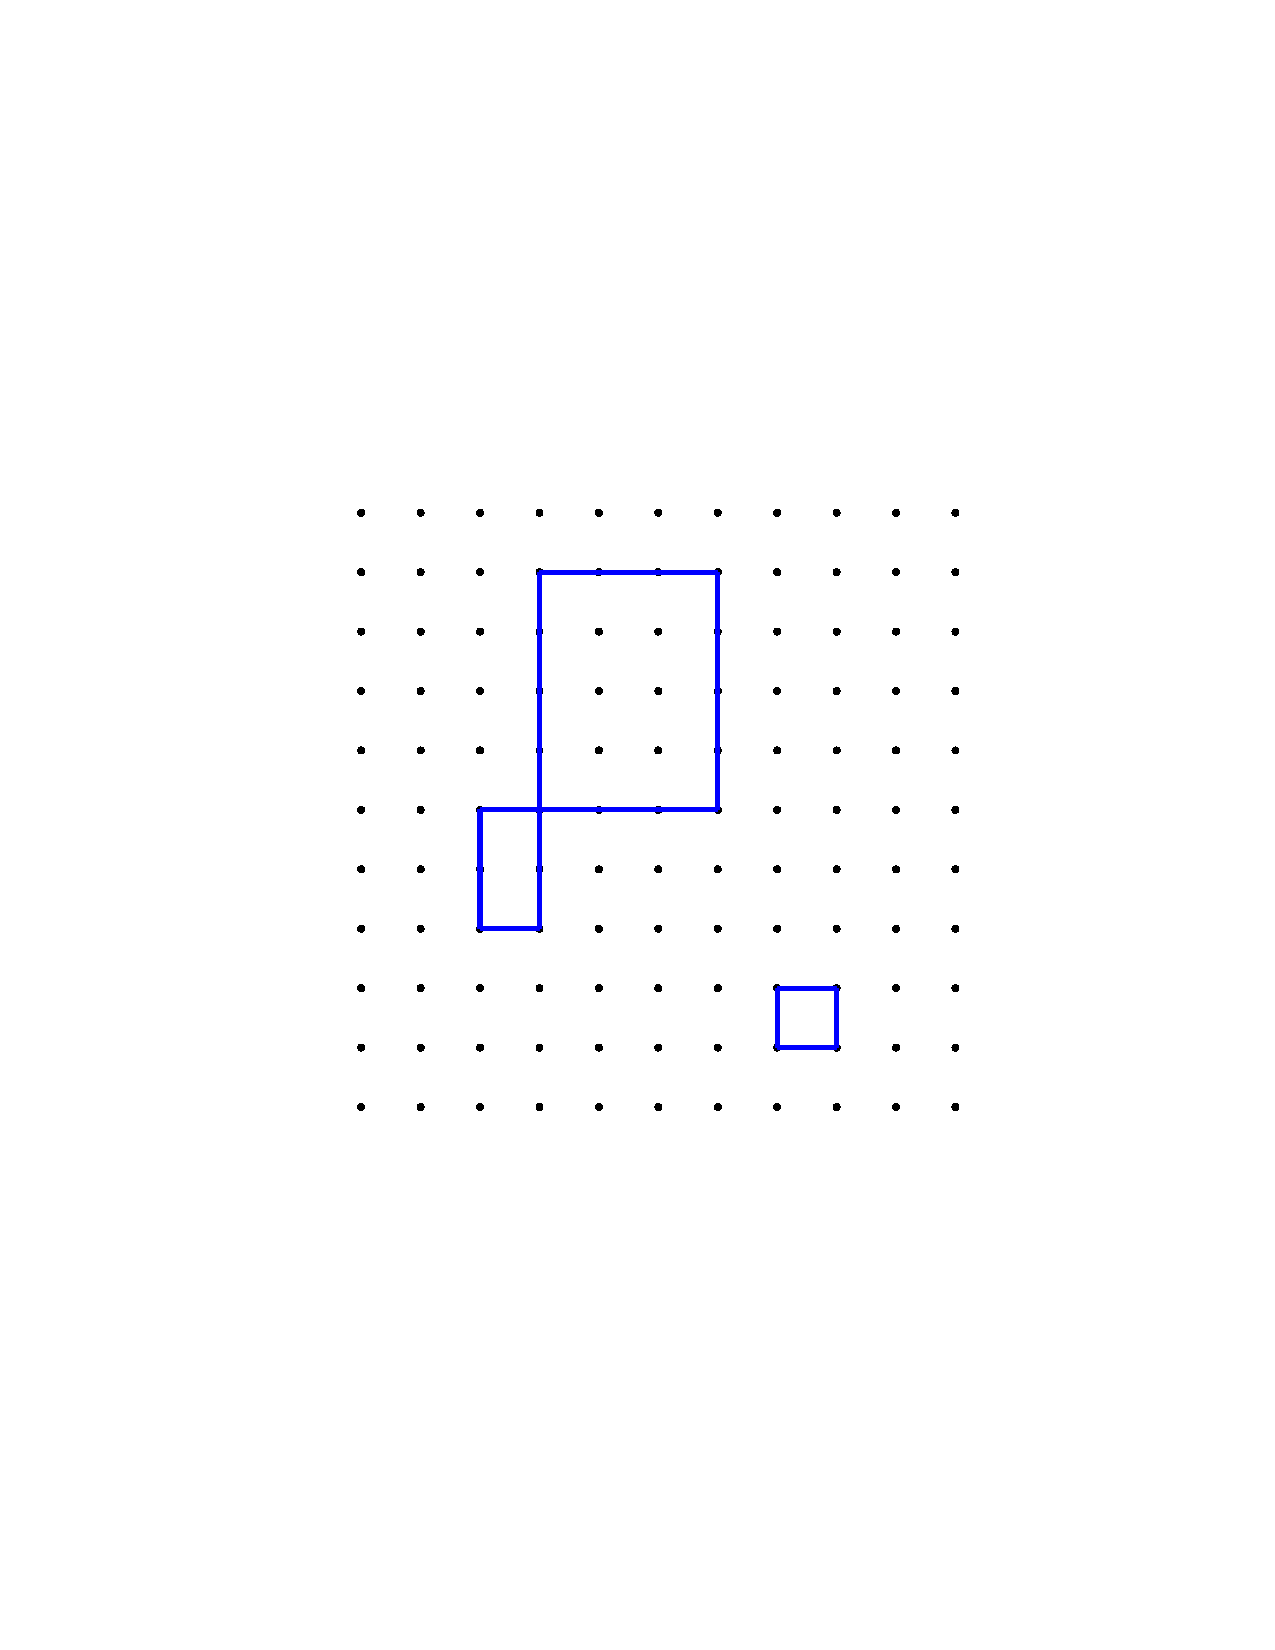
\includegraphics[width=7cm]{Brillouin}
\caption{{\bf .}}
%\label{}
\end{center}
\end{figure}

%
This is the classical limit. 
%
\subsection{Strong spin-orbit coupling}
To avoid confusion we mark operators by hats.
If the spin-orbit coupling is strong compared to the magnetic field, then we cannot ignore the
spin-orbit term. In this case, $H$ still commutes with $L$ and $S$, 
but  no longer with $L^{z}$ and $S^{z}$. Instead, based on the relations
%
\newcommand{\vop}[1]{{\boldsymbol{ \hat #1}}}
\newcommand{\opp}[1]{ \hat {#1} }
\begin{align}
 \vop J &= \vop L + \vop S\\
\vop L\vop S &=\frac{1}{2}\bigg( \vop J^{2}-\vop L^{2}-\vop S^{2} \bigg)\;,\label{eq:para:2}
\end{align}
%
$H$ now commutes  with $L^{2},S^{2},J^{2},J_{z}$. The eigenvectors are therefore
%
\begin{align*}
\ket{\kappa,L,S,J,J_{z}}\;.
\end{align*}
%
The corresponding eigenvalues are given by  \eq{eq:H:spin:orbit:a} as
%
\begin{align*}
E(\kappa,L,S,J,J_{z}) &=E_{0}(\kappa,L,S) + \frac{B \mu_{B}}{\hbar}
\bigg(  J_{z} -\langle \opp S^{z} \rangle \bigg)\;.
\end{align*}
%
Here $\langle \opp S^{z} \rangle$ is the expectation value of of $\opp S^{z}$ in one of the eigenstates
$\ket{\kappa,L,S,J,J_{z}}$, while $J_{z}$ is already the eigenvalue of the operator $\opp J^{z}$.
%
The computation of the expectation value $\avg{\hat S_{z}}$ yields eventually 
%
\begin{align*}
E(\kappa,L,S,J,J_{z} &= E_{0}(\kappa,L,S) + \frac{\mu_{B}B}{\hbar}\underbrace{
\bigg(  1+  \frac{J(J+1)+S(S+1)-L(L+1)}{2 J(J+1)} \bigg)
}_{\color{blue} = g_{J}}J_{z}\\
&= E_{0}(\kappa,L,S) + \mu_{B}B g_{J} m\;,
\end{align*}
%
with $J_{z} = \hbar m$ and $m\in \{-J,-J+1,\dots,J\}$ 

\emphasize{prrof}{
To compute the expectation value we proceed as follows. 
We start out with the  identity
%
\begin{align}\label{eq:para:1}
\vop S \;\big( \vop  L\cdot \vop  S \big) -\big( \vop  L\cdot \vop  S \big)\;\vop  S
&=-i\hbar \vop  S \times \vop L\;.
\end{align}
%
which follows from
%
\begin{align*}
\opp S_{\nu} \;\opp L_{\mu}S_{\mu} - \opp L_{\mu}\opp S_{\mu} \opp S_{\nu} 
&=\opp S_{\nu} \;\opp S_{\mu} \;\opp L_{\mu}-\opp  S_{\mu} \;\opp S_{\nu}\;\opp L_{\mu}
=[\opp S_{\nu} ,\opp S_{\mu}]\;\opp L_{\mu}\\
&=i\hbar \varepsilon_{\nu\mu\rho} \opp S_{\rho} \opp L_{\mu} = -i\hbar \varepsilon_{\nu\rho\mu} \opp S_{\rho} \opp L_{\mu} \\
&=-i \hbar \big( \vop S\times \vop L \big)_{\nu}
\end{align*}\;.
%
%}
Next we multiply \eq{eq:para:1} with $\times \vop  J$ and obtain
%
\begin{align}\label{eq:para:2}
\vop S \;\big( \vop L\cdot \vop S \big)\times \vop J -\big( \vop L\cdot \vop S \big)\;\vop S\times \vop J
&=-i\hbar \big( \vop S\times \vop L \big)\times \vop J
\end{align}
%
Now, $\big( \vop L \cdot   \vop S \big)$ commutes with all components of the vector operator $\vop J$, since
according to \eq{eq:para:2} $\vop L\cdot\vop S$ is given by $\frac{1}{2}(\vop J^{2}-\vop L^{2}-\vop S^{2})$ 
which can be seen as follows
%
\begin{align*}
[\vop L\cdot\vop S,J^{\alpha}] &=
\frac{1}{2}\bigg(\underbrace{[J^{2},J^{\alpha}]}_{\color{blue} = 0}
-[L^{2},J^{\alpha}]-[S^{2},J^{a}]\bigg)\\
&=-\frac{1}{2}\bigg([L^{2},L^{\alpha}+S^{\alpha}]+[S^{2},L^{a}+S^{\alpha}]\bigg)\\
&=-\frac{1}{2}\bigg([L^{2},L^{\alpha}]+[S^{2},S^{\alpha}]\bigg)\\
&=0\;.
\end{align*}
%
Then we can move $\vop L\cdot \vop S$ in the first term of \eq{eq:para:2} to the right of $\vop J$,
resulting in 
%
\begin{align*}
\big(\vop S\times \vop J\big) \;\big( \vop L\cdot \vop S \big)- \big( \vop L\cdot \vop S \big)\;\big(\vop S\times \vop J\big)
&=-i\hbar \big( \vop S\times \vop L \big)\times \vop J
\end{align*}
If we now compute expectation values in the eigenvectors $\ket{\kappa,L,S,J,J_{z}}$, we can replace 
the operators $(\vop L\cdot \vop S)$ by the eigenvalues $\frac{1}{2}\big( J(J+1)-L(L+1)-S(S+1) \big)$ and the remaining expectation value on the left hand side is zero. Hence, we obtain from the right hand side
%
\begin{align}\label{eq:para:3}
\langle \big( \vop S\times \vop L \big)\times \vop J\rangle &= 0\;,
\end{align}
%
which is valid in the eigenstates.
From 
%
\begin{align*}
\big[ \big( \vop S\times \vop L \big)\times \vop J \big]_{i}
&= \varepsilon_{ijk}\big( \vop S\times \vop L \big)_{j} \opp J_{k}\\
&= \varepsilon_{ijk}\varepsilon_{jmn}  \opp S_{m} \opp L_{n} \opp J_{k}\\
&= \varepsilon_{jki}\varepsilon_{jmn}  \opp S_{m} \opp L_{n} \opp J_{k}\\
&= \big( \delta_{km}\delta_{in}-\delta_{kn}\delta_{im} \big)  \opp S_{m} \opp L_{n} \opp J_{k}\\
&= \opp S_{k} \opp L_{i} \opp J_{k}-\opp S_{i} \opp L_{k} \opp J_{k}\\
&= \opp  L_{i} \opp S_{k}\opp J_{k}-\opp S_{i} \opp L_{k} \opp J_{k}\;.
\end{align*}
%
we obtain for the double vector product
%
\begin{align*}
 \big( \vop S\times \vop L \big)\times \vop J &= \vop L\;\big( \vop S\cdot \vop J \big)
 -\vop S\;\big( \vop L\cdot \vop J \big)\\
&=\big( \vop J-\vop S\big)\;\big( \vop S\cdot \vop J \big)
 -\vop S\;\big( \vop L\cdot \vop J \big)\\
&= \vop J\;\big( \vop S\cdot \vop J \big)
 -\vop S\;\big( (\vop L+\vop S)\cdot \vop J \big)\\
 &= \vop J\;\big( \vop S\cdot \vop J \big)
 -\vop S\; \vop J^{2} \;.
\end{align*}
%

From \eq{eq:para:3} we therefore obtain
%
\begin{align*}
 \big( \vop S\times \vop L \big)\times \vop J 
 &= \vop J\;\big( \vop S\cdot \vop J \big)
 -\vop S\; \vop J^{2}  = 0\;.
\end{align*}
%
and for the expectation value in the  eigenstates  $ \ket{\kappa,L,S,J,J^{z}}$
we have
%
\begin{align*}
\avg{ \opp J_{z}\;\big( \vop S\cdot \vop J \big)} -  \avg{\opp  S_{z}\; J^{2} }&=0\;.
\end{align*}
%
Next we use
%
\begin{align*}
\vop S \cdot \vop J &= \vop S \cdot \vop L + \vop S^{2}\\
&=\frac{1}{2}\big( \vop J^{2}-\vop S^{2}-\vop L^{2} \big) + \vop S^{2}\\
&=\frac{1}{2}\big( \vop J^{2}+\vop S^{2}-\vop L^{2} \big) \;.
\end{align*}
and obtain
%
\begin{align*}
 J_{z}\;\frac{1}{2}\avg{ \vop J^{2}+\vop S^{2}-\vop L^{2}}-  \avg{ \opp S_{z}\; J(J+1) }&=0\\
  J_{z}\;\frac{1}{2}\;\big(J(J+1)+S(S+1)-L(L+1)\big) -  \avg{ \opp S_{z}}\; J(J+1)  &=0\;.
\end{align*}
%
%
The expectation value $\avg{S_{z}}$ in the eigenstates  $ \ket{\kappa,L,S,J,J^{z}}$
is therefore:
\begin{align*}
\langle S_{z}\rangle 
&=
J_{z}\; \frac{ J(J+1)+S(S+1)-L(L+1) }{2J(J+1)}\;.
\end{align*}
%
%
Hence, the eigenvalues are
%
\begin{align*}
E(\kappa,L,S,J,J_{z}) &= E_{0}(\kappa,L,S) + \frac{\mu_{B}B}{\hbar}\underbrace{
\bigg(  1+ \frac{1}{2}\big[ J(J+1)+S(S+1)-L(L+1) \big] \bigg)
}_{\color{blue} = g_{J}} J_{z}\;.
\end{align*}
%
}
The remaining calculation is similar to the previous one and one obtains
%
\begin{align*}
\frac{F}{N} 
&= E_{0}
-k_{B}T \ln\bigg(z_{J}\big(b\big) \bigg)
\end{align*}
%
with $b=g_{J}\mu_{B}\beta B$. Then
%
\begin{align*}
\vop M &= \vv e_{z} N J g_{J}\mu_{B}B\;{\cal B}_{J}(b J)\;.
\end{align*}
%

For high $T$ and small $B$, the susceptibility yields
\tboxit{Curie Law}{
%
\begin{align}
\chi_{\mu\nu} &=\delta_{\mu\nu} \frac{C}{T}\;.
\end{align}}
%
with 
%
\begin{align*}
C = \frac{N \mu_{0}\mu_{B}^{2}g_{J}^{2} J(J+1)}{3 k_{B}}\;,
\end{align*}
%
and for large $b$ we have
%
\begin{align*}
\frac{\vv M}{N}
&\underset{b\to\infty}{\longrightarrow} \pm  \vv e_{z} g_{J}\mu_{B}J \;.
\end{align*}

\subsubsection{Plot of the Brillouin function}
\subsubsection{Entropy}
%
For the entropy we obtain
\begin{align*}
\frac{S}{N} &=-\pder{F/N}{T}{\vv B} = k_{B} \ln\big(z_{J}(b)\big)
+k_{B}T \frac{z'_{J}(b)}{z_{J}(b)} \frac{d b}{dT}\\
\end{align*}
%
%
\begin{align*}
 \frac{d b}{dT} &=  -g_{J}\mu_{B} B \frac{1}{k_{B}T^{2}}
 = -\beta^{2} g_{J}\mu_{B} B = - \beta b\;.
\end{align*}
%
\begin{align*}
S &= k_{B} \bigg(\ln\big(z_{J}(b)\big)
-b\frac{z'_{J}(b)}{z_{J}(b)} \bigg)\\
\end{align*}
Along with \eq{eq:para:8} we obtain
\begin{align*}
\frac{S}{N} &= k_{B} \bigg(\ln\bigg(
\frac{\sinh(b (J+1/2))}{\sinh(b/2)}
\bigg)
-b J{\cal B}_{J}(b J) \bigg)\;.
\end{align*}
For  $b \ll 1$ (i.e. $T\to \infty$) we find 
%
\begin{align*}
\frac{S}{N} &=  k_{B} \bigg(\ln\bigg(
\frac{b(J+1/2)}{b/2}
\bigg)
-(b J)^{2} \frac{J+1}{3J}\; \bigg)\\
&=k_{B} \ln\big(2J+1\big)\;.
\end{align*}
%
The argument is the number of eigenvalues of $J_{z}$.
\subsection{Plot of $S$ and specific heat}
\section{Magnetism of the free electron model}
The free electron gas is based on the following assumptions: no electron-electron interactions, 
the electrons experience no potential due to the crystal, they  are confined to a box. In addition,
we apply a constant homogeneous external magnetic field. 


\subsection{Pauli paramagnetism}

First, we restrict the discussion to the coupling of the electronic spin to the magnetic field, i.e.
we ignore the angular moment.
The energy one-particle eigenvalues are
%
\begin{align*}
\varepsilon_{\sigma}(\vv k) &= \frac{\hbar^{2} \vv k^{2}}{2m} +\sigma b\;,\\
b &= \frac{\mu_{B} g_{e} }{2}B\;.
\end{align*}
%
with the quantized wave vectors $\vv k$.
The mean occupation of the one-particle orbitals is given by the Fermi-Dirac distribution
%
\begin{align*}
n_{F}(\varepsilon_{\sigma}(\vv k)|T,\mu)
\end{align*}
%
The mean total number of electrons in the Zeeman level represented by $\sigma$ is
%
\begin{align*}
N_{\sigma} &=\sum_{\vv k} n_{F}(\varepsilon_{\sigma}(\vv k)|T,\mu)
= \int d\varepsilon \rho(\varepsilon) n_{F}(\varepsilon +\sigma b|T,\mu)\;.
\end{align*}
%
As derived in \app{app:dos} the 3D dos is
%
%
\begin{subequations}\label{eq:para:pauli:1}
\begin{align}
\rho(\varepsilon)&= D \sqrt{\varepsilon}\;,\\
\text{with}\quad D&=\frac{V m^{3/2}}{\hbar^{3} \pi^{2}\sqrt{2}}\;.
\end{align}
\end{subequations}
%
Then
%
\begin{align*}
N_{\sigma} &=D\;
\int_{0}^{\infty} d\varepsilon \sqrt{\varepsilon} \; n_{F}(\varepsilon +\sigma b|T,\mu)\;.
\end{align*}
%
For small magnetic field we can use a Taylor expansion in $b$ abound $b=0$
%
\begin{align*}
N_{\sigma} &=D\;
\int_{0}^{\infty} d\varepsilon \sqrt{\varepsilon} \; 
\bigg(n_{F}(\varepsilon|T,\mu) +\sigma b \;\frac{\partial }{\partial \varepsilon}n_{F}(\varepsilon|T,\mu) +{\cal O}(b^{2})\bigg)\\
 &=D\;
\int_{0}^{\infty} d\varepsilon \sqrt{\varepsilon} \; 
n_{F}(\varepsilon|T,\mu) 
+\sigma b D \int_{0}^{\infty} d\varepsilon \sqrt{\varepsilon} \;n'_{F}(\varepsilon|T,\mu) +{\cal O}(b^{2})
\end{align*}
%
 The total particle number follows as
 %
\begin{align}
N &= N_{+}+N_{-} = 2 D \int_{0}^{\infty} d\varepsilon \sqrt{\varepsilon} \;n_{F}
(\varepsilon|T,\mu) +
{\cal O}(b^{2})\notag\\
&= 2 D \int_{0}^{\infty} d\varepsilon \sqrt{\varepsilon} \;n_{F}
(\varepsilon|T,\mu) +
{\cal O}(b^{2})\;.\label{eq:N:total}
\end{align}
%
For small $b$ and low temperature we can use the Sommerfeld expansion, outlined in \app{Sommerfeld},
%
\tboxit{Sommerfeld expansion}{
\begin{align}\label{eq:}
I&=\int_{0}^{\infty}  f(\varepsilon) n_{F}(\varepsilon|\mu,T) d\varepsilon\nonumber\\
 &=\int_{0}^{\mu} f(\varepsilon)d\varepsilon
+ 2  \sum_{n=1}^{\text{odd}}\big(1-\frac{1}{2^{n}}\big)\;\zeta(n+1)
\big(k_{B}T\big)^{n+1}\;f^{(n)}(\mu)\;,
\end{align}}
%
which reads to leading order
%
\begin{align*}
I &= \int_{0}^{\mu} f(\varepsilon) d\varepsilon +  \frac{\pi^{2}}{6}\;\big(k_{B}T\big)^{2} \;f'(\mu)+ {\cal O}(\big(\frac{k_{B}T}{\mu}\big)^{4})\;.
\end{align*}
%
For the total particle number we obtain
\begin{align*}
N&=2 D \bigg(\int_{0}^{\mu}\sqrt{\varepsilon} 
+\frac{\pi^{2}}{6}\frac{d}{d\mu}\sqrt{\mu}\bigg( k_{B}T \bigg)^{2}+\ldots\bigg)\\
&=2 D \bigg(\frac{2}{3}\mu^{3/2} 
+\frac{\pi^{2}}{12}\mu^{-1/2}\big( k_{B}T \big)^{2}+\ldots
\bigg)\;.
\end{align*}
%
%
\begin{align}\label{eq:spin:para:aux2}
\frac{3 N}{4 D}&= \mu^{3/2}\bigg(1
+\frac{\pi^{2}}{8}\bigg(\frac{ k_{B}T }{\mu}\bigg)^{2}+\ldots
\bigg)
\end{align}
%

%
For $T=0$ the chemical potential is equivalent to the Fermi energy $\varepsilon_{F}$ and we have
%
\begin{align}\label{eq:spin:para:aux1}
\frac{3 N}{4 D} &= \varepsilon_{F}^{3/2}\;,
\end{align}
%
or rather
%
\begin{align*}
\varepsilon_{F} 
&=  \bigg(\frac{3 N \hbar^{3}  (2\pi)^{2} }{4 V(2m)^{3/2}} \bigg)^{2/3}
=  \bigg(\frac{3 N   \pi^{2} }{ V} \bigg)^{2/3}\;\frac{\hbar^{2}}{2 m}\;.
\end{align*}
%
\tboxit{Fermi energy in the free electron gas}{
\begin{align}\label{eq:spin:para:EF}
\varepsilon_{F}&=  \bigg(3  \pi^{2} n\bigg)^{2/3}
\frac{\hbar^{2}}{2m} \;.
\end{align}}
%
This defines the Fermi wave number $k_{F}$, through
%
\begin{align*}
\varepsilon_{F} &
= \bigg(3  \pi^{2} n\bigg)^{2/3}\frac{\hbar^{2}}{2m} 
= \frac{\hbar^{2}	k_{F}^{2} }{2m}\\
k_{F}&=\bigg(3  \pi^{2} n\bigg)^{1/3} = \bigg(\frac{3 \pi^{2}}{v}\bigg)^{1/3 }\;,
\end{align*}
%
where $v$ is the average volume per electron. Hence 
%
\begin{align*}
k_{F} &\propto \frac{1}{r}\;,
\end{align*}
%
where $r$ is the mean distance between the electrons.
Inserting \eq{eq:spin:para:aux1} in \eq{eq:spin:para:aux2} yields apart from higher order terms
%
\begin{align*}
\varepsilon_{F}
&= \mu\bigg(1 +\frac{\pi^{2}}{8}\bigg(\frac{ k_{B}T }{\mu}\bigg)^{2}\bigg)^{2/3}\\
\mu &= \varepsilon_{F}\bigg(1 +\frac{\pi^{2}}{8}\bigg(\frac{ k_{B}T }{\mu}\bigg)^{2}\bigg)^{-2/3}\;.
\end{align*}
%
We can solve this equation iteratively, starting with 
$\mu=\varepsilon_{F}$. The first iteration yields
%
\begin{align*}
\mu &=\varepsilon_{F}\bigg(1 +\frac{\pi^{2}}{8}\bigg(\frac{ k_{B}T }{\varepsilon_{F}}\bigg)^{2}\bigg)^{-2/3}\;.
\end{align*}
%
For low temperatures, 
$\frac{ k_{B}T }{\varepsilon_{F}}<1$ we can as well write
\begin{align*}
\mu &=\varepsilon_{F}\bigg(1 -\frac{\pi^{2}}{8}\frac{2}{3}\bigg(\frac{ k_{B}T }{\varepsilon_{F}}\bigg)^{2} +{\cal O}\bigg( \big( \frac{k_{B}T}{\varepsilon_{F}} \big)^{4} \bigg)\bigg)\;.
\end{align*}
%
Further iterations do not change the second order term and we generally have
%
\tboxitp{Chemical potential}{free electron gas}{
\begin{align}\label{eq:}
\mu &=\varepsilon_{F}\bigg(1 -\frac{\pi^{2}}{12}\bigg(\frac{ k_{B}T }{\varepsilon_{F}}\bigg)^{2} \bigg)\;+{\cal O}\bigg( \big( \frac{k_{B}T}{\varepsilon_{F}} \big)^{4} \bigg)
\end{align}}
%

%

%
The partition function for non-interacting particles has already been derived previously.
For one-particle energies $\varepsilon_{\nu}$ it was
%
\begin{align*}
\ln(Z) &= \sum_{\nu} \ln\bigg( 1+  e^{-\beta(\varepsilon_{\nu}-\mu)}\bigg)\;.
\end{align*}
%
In the present case the index $\nu$ stands for the wave vector $\vv k$ and the spin direction. Hence
%
\begin{align}\label{eq:para:pauli:ln:Z}
\ln(Z) 
%&= \sum_{\sigma} \sum_{\vv k} \ln\bigg( 1+  e^{-\beta(\varepsilon(\vv k)+\sigma b-\mu)}\bigg)\\
&= \sum_{\sigma} \int_{0}^{\infty}\;\rho(\varepsilon)\;
\ln\bigg( 1+  e^{-\beta(\varepsilon+\sigma b-\mu)}\bigg)\;.
\end{align}
%

The corresponding grand  potential reads
%
\begin{align*}
\Omega(T,\vv B) &= -k_{B}T \ln(Z) =-k_{B}T   \sum_{\sigma} \int_{0}^{\infty}\;\rho(\varepsilon)\;
\ln\bigg( 1+  e^{-\beta(\varepsilon+\sigma b-\mu)}\bigg)\;.
\end{align*}
%
The magnetization in z-direction is obtain via
%
\begin{align*}
M &= - \pder{\Omega}{B}{T} \\
&=k_{B}T\;\sum_{\sigma}\big( -\frac{\beta\sigma \mu_{B}g_{e}}{2} \big)
\int_{0}^{\infty} d\varepsilon\;\rho(\varepsilon)\;\frac{e^{-\beta(\varepsilon+\sigma b-\mu)}}{1+e^{-\beta(\varepsilon+\sigma b-\mu)}}\\
&=-\frac{\mu_{B}g_{e}}{2} \;\sum_{\sigma}\sigma \;\;
\int_{0}^{\infty} d\varepsilon\;\rho(\varepsilon)\;n_{F}(\varepsilon+\sigma b|T,\mu)\\
&= -\frac{\mu_{B}g_{e}}{\hbar} \;\underbrace{
 \frac{\hbar(N_{+}-N_{-})}{2}
}_{\color{blue} = \langle S_\text{total}^{z} \rangle}
\end{align*}
%
In agreement with \eq{eq:magmo:spin}. Again we assume that $b$ is small and 
employ a Taylor expansion. 
%
\begin{align*}
M &= -\frac{\mu_{B}g_{e} }{2} \sum_{\sigma} \sigma \int_{0}^{\infty}d\varepsilon \bigg(\rho(\varepsilon) n_{F}(\varepsilon|T,\mu) + \sigma b n'_{F}(\varepsilon|T,\mu)+{O}(b^{2})\bigg)\\
&= -\frac{\mu_{B}g_{e} }{2} 2b \int_{0}^{\infty}d\varepsilon \rho(\varepsilon)  n'_{F}(\varepsilon|T,\mu)+{O}(b^{2})\\
&= -\frac{(\mu_{B}g_{e})^{2} }{2}  B\int_{0}^{\infty}d\varepsilon \rho(\varepsilon)  n'_{F}(\varepsilon|T,\mu)+{O}(b^{2})\;.
\end{align*}
%
Then the susceptibility reads
%
\begin{align}
\chi_{T} &= \mu_{0}\pder{M}{B}{T}\bigg|_{B=0}\notag\\
&=-\mu_{0}\frac{(\mu_{B}g_{e})^{2} }{2}  \int_{0}^{\infty}d\varepsilon \rho(\varepsilon)  n'_{F}(\varepsilon|T,\mu)\notag\;.
\end{align}
%
This can also be written as
%
\begin{align*}
\chi_{T} &= -\mu_{0} \mu_{B}^{2} \bigg(\frac{g_{e}}{2}\bigg)^{2} 2 
\int d\varepsilon \rho(\varepsilon) n'_{F} (\varepsilon|T,\mu)\\
&= \mu_{0} \mu_{B}^{2} \bigg(\frac{g_{e}}{2}\bigg)^{2} 2 
\frac{\partial }{\partial \mu} 
\int d\varepsilon \rho(\varepsilon) n_{F} (\varepsilon|T,\mu)\;.
\end{align*}
%
Comparison with \eq{eq:N:total} yields 
\begin{align}\label{eq:Pauli:dN:dmu}
\chi_{T} 
&= \mu_{0} \mu_{B}^{2} \bigg(\frac{g_{e}}{2}\bigg)^{2} 
\pder{N}{\mu}{T,B=0}
\end{align}

We use the Sommerfeld expansion, derived in \app{Sommerfeld} to expand the integral in powers of $k_{B}T/\mu$. 
%
\begin{align*}
\chi &=-\mu_{0}\frac{(\mu_{B}g_{e})^{2} }{2}  \int_{0}^{\infty}d\varepsilon \rho(\varepsilon)  n'_{F}(\varepsilon|T,\mu)\notag\\
&=\mu_{0}\frac{(\mu_{B}g_{e})^{2} }{2}  \int_{0}^{\infty}d\varepsilon \rho'(\varepsilon)  n_{F}(\varepsilon|T,\mu)\\
 &=\mu_{0}\frac{(\mu_{B}g_{e})^{2} }{2}  \bigg(\int_{0}^{\mu}d\varepsilon \rho'(\varepsilon)
+\frac{\pi^{2}}{6}(k_{B}T)^{2}\rho''(\mu)+ {\cal O}(\big(\frac{k_{B}T}{\mu}\big)^{4})
 \bigg)\\    
  &=\mu_{0}\frac{(\mu_{B}g_{e})^{2} }{2}  \bigg( \rho(\mu)
+\frac{\pi^{2}}{6}(k_{B}T)^{2}\rho''(\mu)+ {\cal O}(\big(\frac{k_{B}T}{\mu}\big)^{4})
 \bigg)\;.
\end{align*}
%
The final result reads
%
\begin{align}\label{eq:para:chi}
\chi   &=\mu_{0}\frac{(\mu_{B}g_{e})^{2} }{2}  \rho(\mu)\bigg( 1
+\frac{\pi^{2}}{6}(k_{B}T)^{2}\frac{\rho''(\mu)}{\rho(\mu)}+\ldots
 \bigg)
\end{align}
%
Now we recall, that $\rho(\varepsilon) = D \sqrt{\varepsilon}$, resulting in
$\rho''(\mu)/\rho(\mu)=-1/(4\mu^{2})$. 
%
\tboxitp{Magnetic susceptibility}{free electron gas}{
\begin{align}
\chi_{P} &= \mu_{0}\frac{(\mu_{B}g_{e})^{2} }{2}  \rho(\mu)
\bigg( 1 - \frac{\pi^{2}}{24}\bigg(\frac{k_{B}T}{\mu}\bigg)^{2} +\ldots\bigg)\;.
\end{align}}
%
We see that indeed $k_{B}T/\mu$ is the relevant small parameter.
This describes the \red{Pauli-spin-paramagnetism}, which is almost temperature
independent for low $T$; in strong contrast to the Curie $1/T$ behaviour.
The reason for the discrepancy lies in the fermi-statistics. Only the spin of the electrons in the vicinity of $\mu$ can contribute. The number of thermally excited electrons
is $k_{b} T \rho(\mu)$ which compensates the $1/T$ behaviour.


\subsection{Langevin Diamagnetismus}
So far we have only considered the spin degrees of freedom of the free electron gas. The orbital moments also contribute to the magnetization, which results in the
\tboxitp{Landau Diamagnetism}{free electron gas}{
%
\begin{align}\label{eq:}
\chi_{L}&= -\frac{1}{3}\chi_{P}
\end{align}
%
}
For the derivation see appendix \ref{app:free:electron:gas}


\section{Collective magnetism }

\subsection{Heisenberg hamiltonian}
In many crystaline  systems, the electrons can be split into those that are localized at the atomic sites and others which can move freely through the crystal. The former result in localized
magnetic moments or spins $\vv S_{i}$, if they do not belong to closed shells. 
We have discussed these  local spins $\vv S_{i}$ before, but there we have focussed on systems where these spins do not interact. 
The Coulomb interaction between the electrons can lead to various types of exchange interactions
between these spins. The exchange can either result from exchange processes of the electrons that form the local spins on neighboring sites {\em direct exchange} or it can be mediated by
additional electrons {\em indirect exchange}. In the latter case, the interaction can be long ranged, like in the case of the so-called {\em RKKY} (Ruderman-Kittel-Kasuya-Yosida). 
In RKKY the interaction decays like $1/\abs{\vv R_{i}-\vv R_{j}}^{3}$ with the distance between the spins at site 
$\vv R_{i}$ and $\vv R_{j}$. In addition, the exchange interaction  changes sign as function of distance, i.e.
depending on the distance between the localized spins it can be ferromagnetic and anti-ferromagnetic. In all cases, the interaction can be described by a prominent model for collective magnetism, the 
\tboxit{Heisenberg model}{
\begin{align}\label{eq:}
H &= - \sum_{jj'}
\bigg( J^{z}_{jj'} S^{z}_{j}   S^{z}_{j'}+  J^{xy}_{jj'} 
\big(S^{x}_{j}   S^{x}_{j'}+ S^{y}_{j}   S^{y}_{j'}\big)
\bigg) 
+ b \sum_{j} S^{z}_{j}\;.
\end{align}
}
Here $J_{jj'} = J((\vv R_{j}-\vv R_{j'}))$, with $J_{jj}=0$.
 $J_{jj'}$ can always be chosen symmetric, since by substituting $j\leftrightarrow j'$ we find
%
\begin{align*}
H_{H}= -\sum_{\alpha}\sum_{jj'} J_{jj'} S^{\alpha}_{j}S^{\alpha}_{j'} &= -\sum_{\alpha}\sum_{jj'} J_{j'j} S^{\alpha}_{j'}S^{\alpha}_{j} =-\sum_{\alpha}\sum_{jj'} J_{j'j} S^{\alpha}_{j}S^{\alpha}_{j'} 
\end{align*}
%
Hence 
%
\begin{align*}
H &= \frac{1}{2}\bigg(  -\sum_{\alpha}\sum_{jj'} J_{jj'} S^{\alpha}_{j}S^{\alpha}_{j'} 
+ -\sum_{\alpha}\sum_{jj'} J_{j'j} S^{\alpha}_{j}S^{\alpha}_{j'}  \bigg)=
 -\sum_{\alpha}\sum_{jj'} \big(\frac{J_{jj'}+J_{j'j}}{2}\big) S^{\alpha}_{j}S^{\alpha}_{j'} \;.
\end{align*}
%
We also introduce the ladder operators
%
\begin{align}\label{eq:}
S_{j}^{\pm} &= S_{j}^{x}\pm i S_{j}^{y}\;.
\end{align}
%
In these operators, the hamiltonian reads
\begin{align*}
H &= - \sum_{jj'} \bigg( J^{z}_{jj'} S_{j}^{z}  S_{j'}^{z}
+J_{jj'}^{xy}S_{j}^{+} S_{j'}^{-}
\bigg) + b \sum_{j} S^{z}_{j}\;.
\end{align*}
%
The order of the operators $S_{j}^{+}S_{j'}^{-}$ is irrelevant, since $j\ne j'$ and in that case they commute.
There are three important limiting cases depending on the anisotropy of the crystal in spin-space.
\begin{itemize}
	\item ($\abs{J^{z}}\ll\abs{J^{xy}}$) results in the so-called {\em xy- model}
\tboxit{xy-model}{
\begin{align}
H &= - \sum_{jj'} 
J_{jj'}^{xy}S_{j}^{+} S_{j'}^{-}
 + b \sum_{j} S^{z}_{j}\;.
\end{align}}

\item ($\abs{J^{z}}\gg\abs{J^{xy}}$) results in the so-called {\em Ising model}, which is discussed in great detail chapter \chap{chap:ising}
\item ($J^{z} = J^{xy}$)  represents the isotropic Heisenberg model

%
\tboxitp{Heisenberg model}{isotropic case}{
\begin{align}\label{eq:heisenberg}
H &= - \sum_{jj'} J_{jj'} \vv S_{j}  \vv S_{j'} + b \sum_{j} S^{z}_{j}\;.
\end{align}
}
\end{itemize}
%
Very often the exchange coupling $J_{jj'} = J(\abs{\vv R_{j}-\vv R_{j'}})$ decreases
very rapidly with distance and it suffices to take only nearest neighbour (nn) interactions into account, i.e.
%
\begin{align}\label{eq:}
-\sum_{jj'} J_{jj'} \approx -J \sum_{\langle jj' \rangle}\;.
\end{align}
%
In general, $J$ can be positive or negative. In the first (second) case,  ferromagnetic (anti-ferromagnetic) spin alignment is favoured. If the exchange coupling between localized spins
is mediated by itinerant electrons, the so-called {\em RKKY-interaction} (Ruderman-Kittel-Kasuya-Yosida) results, which is long ranged and oscillating as function of distance, i.e.
depending on the distance between the localized spins it can be ferromagnetic and anti-ferromagnetic.
\subsection{Mermin-Wagner Theorem}
%
There are only a few exact results available for the Heisenberg model. Presumably the most important one is due to Mermin and Wagner and states:
\red{\em In one and two dimensions, continuous symmetries cannot be  broken spontaneously at finite temperature in systems with sufficiently short-ranged interactions.}

We add an external field 
 %
\begin{align*}
\vv B_{j} &= b \vv e_{z} e^{i \vv Q \vv R_{j}}\;,
\end{align*}
%
to the isotrop ferromagnetic Heisenberg model.
This B-field  couples to different types of magnetic order (e.g. ferro, anti-ferro), depending on the choice of the wave vector $\vv Q$. 
%
We consider the order parameter 
%
\begin{align}
{\cal S}_{\vv Q}(T,b) &= \frac{1}{\hbar N}\langle \vv S^{z}_{\vv Q}\rangle_{T,b}\;.
\end{align}

The operator $S^{z}_{\vv Q}$ stands for the Fourier transform of $S_{j}^{z}$, defined in \eq{eq:FT:magnetism}.

After a straightforward but tedious calculation, which can be found in appendix \ref{app:mermin:wagner}, the result reads
%

\begin{subequations}\label{eq:}
\begin{align}
1D) &&\abs{{\cal S}_{\vv Q}(T,b)}&\le \bigg(\frac{  \abs{b}}{T^{2}}\bigg)^{1/3} &&\underset{b\to 0}{\longrightarrow} 0\\
2D) &&\abs{{\cal S}_{\vv Q}(T,b)}&\le 
\frac{const}{\sqrt{T
  \big|  \ln\big( \abs{b}  \big)\big| }}&&\underset{b\to 0}{\longrightarrow} 0\\
3D) &&  \abs{{\cal S}_{\vv Q}(T,b)} &\le \frac{const}{\sqrt{T}}
\end{align}
\end{subequations}
%
For finite $T$ the rhs in 1D 2D goes to zero for vanishing field ($b\to 0$).
Hence there is no finite order parameter possible, irrespective of the wve vector $\vv Q$ (order). 
For 3D, however, the Mermin-Wagner theorem does not rule out spontaneous  magnetization for finite $T$.



 
 \subsection{Exact ground-state of the ferromagnetic Heisenberg model}

Here we consider only the \red{homogeneous}  ferromagnetic ($J_{jj'}>0$) Heisenberg model
with a homogenous magnetic field pointing in the $z$-direction.
We readily see that the ground state is given by the 
state, where all spins are maximally aligned in the negative $z$-direction
%
\begin{align}\label{eq:}
\ket{0} &= \otimes_{j=1}^{N} \ket{-S}_{j}
\end{align}
%
with
\begin{subequations}\label{eq:}
\begin{align}
S_{j}^{z} \ket{m}_{j} &=\hbar m \ket{m}_{j}\\
S_{j}^{2} \ket{m}_{j} &=\hbar^{2} S(S+1) \ket{m}_{j}\;.
\end{align}
\end{subequations}
Applying the hamiltonian to $\ket{0}$ yields
%
\begin{align*}
H\ket{0} &= - \sum_{jj'} J_{jj'} S_{j}^{z}  S_{j'}^{z}\ket{0}
- \sum_{jj'} J_{jj'} S_{j}^{+} \underbrace{
S_{j'}^{-}\ket{0}
}_{\color{blue} = 0}
\bigg) + b \sum_{j} S^{z}_{j}\ket{0}\\
&= - \sum_{jj'} J_{jj'} \hbar^{2} S^{2}  \ket{0} - b \sum_{j} \hbar S \ket{0}\\
&=-\hbar  \bigg(N \sum_{l} J(|\vv R_{l}|) \hbar  S^{2}  + b \sum_{j}  S \bigg)\ket{0}\\
&=-\hbar  N \bigg(\hbar \tilde J(0)  S^{2}  + b   S \bigg)\ket{0}\\
\tilde J(0) &=  \sum_{l} J(|\vv R_{l}|) \;.
\end{align*}
%
We have introduced the Fourier transform of the exchange coupling.
%
\begin{align}\label{eq:heisenberg:J:q}
\tilde J(\vv k) &= \sum_{l} J(|\vv R_{l}|) e^{i \vv k \vv R_{l}}\;.
\end{align}
%
Obviously, $\ket{0}$ is an eigenvector.
We consider
%
\begin{align*}
\big( \vv S_{j} + \vv S_{j} \big)^{2} &= \vv S_{j}^{2}+\vv S_{j'}^{2} + 2 \vv S_{j} \vv S_{j'}\\
- \vv S_{j} \vv S_{j'} &= \frac{1}{2}\big(\vv S_{j}^{2}+\vv S_{j'}^{2} \big)- 
\frac{1}{2}\big( \vv S_{j} + \vv S_{j} \big)^{2}
\end{align*}
%
All spins have magnitude $S$. We consider an arbitrary vector $\ket{\psi}$, which is an eigenstate 
of all $\vv S_{j}^{2}$  with eigenvalue $S(S+1)$ but otherwise arbitrary. Then
\begin{align*}
- \avg{\vv S_{j}} \vv S_{j'} &= S(S+1) 
- \frac{1}{2}\avg{\big( \vv S_{j} + \vv S_{j} \big)^{2}}
\end{align*}
Now $\vv S' :=\vv S_{j} + \vv S_{j}$ is an effective spin where the eigenvalues of
$\vv S'^{2}$ are given bei $S'(S'+1)$ with $S'\in \hbar \{0,1,\ldots,2 S\}$.
Consequently,
%
\begin{align*}
\frac{1}{2}\avg{\big( \vv S_{j} + \vv S_{j} \big)^{2}} \le 2S(2S+1)\;.
\end{align*}
%
Then
%
\begin{align*}
- \avg{\vv S_{j}} \vv S_{j'} &\ge S(S+1)  S(2S+1) = S^{2}
\end{align*}
%
Finally that means if $J_{jj'}\ge 0 \forall j,j'$
%
\begin{align*}
\avg{H_{0}} &= \sum_{jj'} J_{jj'} \bigg(-\avg{\vv S_{j}} \vv S_{j'}\bigg) \\
&\ge -S^{2}\hbar^{2}\;\sum_{jj'} J_{jj'}\\
\avg{H_{0}} &\ge - N \hbar^{2} \tilde J(0)\;.
\end{align*}
%
For the Zeeman term we see readily
%
\begin{align*}
\avg{H_{Z}} &\ge  - b S\hbar 
\end{align*}
%
Hence in total we have for the energy

%
\begin{align*}
E &\ge - N \hbar^{2} \tilde J(0) - b S\hbar = E_{0}
\end{align*}
%
Since there is no energy lower than the ferromagnetic state, it is the groundstate.
Moreover, we see that 
%
\begin{align*}
S^{z}_{total} &=\sum_{j} \vv S_{j}^{z}\ket{0} = \hbar NS \ket{0}\;.
\end{align*}
%
The groundstate is an eigenstate of $S^{z}_{total}$ and also of
%
\begin{align*}
\vv S_{total}^{2} &=\sum_{j\ne j'} \vv S_{j} \vv  S_{j'} + \sum_{j} \vv S_{j}^{2}\\
\vv S_{total}^{2}\ket{0} &=\sum_{j\ne j'} \vv S_{j} \vv  S_{j'}\vv S_{total}^{2}\ket{0} + N 
\hbar^{2}S(S+1)\ket{0}\\
\vv S_{total}^{2}\ket{0} &=\sum_{j\ne j'} \hbar^{2}S^{2} \ket{0} + \underbrace{
S_{j}^{+} S_{j'}^{-} \ket{0}
}_{\color{blue} = 0} + NS(S+1)\hbar^{2} \ket{0}\\
&=\bigg( N(N-1)\hbar^{2} S^{2} +  NS(S+1)\hbar^{2}\bigg)\ket{0}\\
&=\hbar^{2}\bigg( N^{2} S^{2} - \canceled{N  S^{2}} +  \canceled{N S^{2}} + NS \bigg)\ket{0}\\
&=\hbar^{2}\; N S\big(NS+1  \big) \ket{0}
\end{align*}
%
So it $\ket{0}$ an eigenstate of $\vv S_{total}$ with maximum magnitude $NS\hbar$.

\subsection{Spin waves in the ferromagnetic Heisenberg model}
%
Next we study the low-laying excited states. To this end we 
first consider the  hamiltonian in  Fourier space. 
The details of the 
Fourier transform as introduced in \eq{eq:FT:magnetism} are
\begin{subequations}\label{eq:FT:magnetism2}
\begin{align}
S_{k}^{\alpha} &= \sum_{j} S_{j}^{\alpha} e^{i \vv k \vv R_{j}}\;,\qquad \alpha\in\{x,y,z\}\\
S_{j}^{\alpha}&=\frac{1}{N} \sum_{k}^{1.Bz} S_{k}^{\alpha} e^{-i \vv k \vv R_{j}}
\end{align}
\end{subequations}
%
We recall the commutation relations 
%
\begin{subequations}\label{eq:}
\begin{align}
\big[ S_{j}^{\alpha}S_{j'}^{\beta}	 \big] &= \delta_{jj'}
i \hbar \varepsilon_{\alpha\beta\gamma}S_{j}^{\gamma}\;,\\
\big[S_{j}^{z} S^{\pm}_{j'}\big] &=\pm \delta_{jj'} \hbar S^{\pm}_{j}\;,\\
\big[S^{-}_{j},S^{+}_{j'}\big] 
&= -2 \hbar \delta_{jj'} S^{z}_{j}\;,\\
\big[S^{+}_{j},S^{+}_{j'}\big]  &= 0\;.
\end{align}
\end{subequations}
Then
%
\begin{subequations}\label{eq:}
\begin{align}
\big[S_{\vv k}^{z} S^{\pm}_{\vv k'}\big] 
&=\pm  \hbar S^{\pm}_{\vv k+\vv k'}\;,\\
%%%%
\big[S^{-}_{\vv k},S^{+}_{\vv k'}\big] 
&= -2 \hbar S^{z}_{\vv k +\vv k'}\;,\\
\big[S^{+}_{j},S^{+}_{j'}\big]  &= 0\;.
\end{align}
\end{subequations}



%\emphasize{Proof}{
%
\begin{align*}
\big[S_{j}^{z} S^{\pm}_{j'}\big] &=\big[S_{j}^{z} S^{x}_{j'}\big] \pm i
\big[S_{j}^{z} S^{y}_{j'}\big]\\
&=\delta_{jj'}
i \hbar \bigg( \varepsilon_{z x y} S^{y}_{j}
\pm i \varepsilon_{z y x} S^{x}_{j}\\
&=\delta_{jj'}
 \hbar \bigg(i \underbrace{
\varepsilon_{z x y}
}_{\color{blue} = +1} S^{y}_{j}
\mp  \underbrace{
\varepsilon_{z y x}
}_{\color{blue} = -1} S^{x}_{j}
\bigg)\\
&= \delta_{jj'} \hbar \bigg(i S^{y}_{j} \pm  S^{x}_{j}\bigg)\\
&=\pm \delta_{jj'} \hbar \bigg(S^{x}_{j} \pm i S^{y}_{j}   \bigg)\;.
\end{align*}
%
%
\begin{align*}
\big[S_{\vv k}^{z} S^{\pm}_{\vv k'}\big] 
&=
\sum_{jj'}e^{i\big(\vv k \vv x_{j} + \vv k' \vv x_{j'}\big)}
\big[S_{j}^{z} S^{\pm}_{ j'}\big] 
\\
&=\pm \hbar 
\sum_{jj'}e^{i\big(\vv k \vv x_{j} + \vv k' \vv x_{j'}\big)}
\delta_{jj'} S^{\pm}_{j}\\
&=\pm  \hbar 
\sum_{j}e^{i\big(\vv k + \vv k' \big)\vv x_{j}} S^{\pm}_{j}\\
%%%%
&=\pm  \hbar S^{\pm}_{\vv k+\vv k'}\;.
\end{align*}
%
%
\begin{align*}
\big[S^{-}_{j},S^{+}_{j'}\big] 
&=\big[\big(S^{x}_{j}- iS ^{y}_{j}\big),\big(S^{x}_{j'}+ i S^{y}_{j'}\big)\big] \\
&=i \big[S^{x}_{j},S^{y}_{j'}\big]
 -  \big[S^{y}_{j},S^{x}_{j'}\big]\\
&= 2 i  \delta_{jj'} \big(i \hbar S_{j}^{z}\big)\\
&= - 2  \hbar \delta_{jj'}  S_{j}^{z}\;.
\end{align*}
%
%
\begin{align*}
\bigg[S^{-}_{\vv k},S^{+}_{\vv k'}\bigg] &= \sum_{jj'}
e^{i\big(\vv k \xx{j}+\vv k' \xx{j'}\big)}
\underbrace{
\big[S^{-}_{j},S^{+}_{j'}\big]
}_{\color{blue} = - 2\hbar \delta_{jj'}S^{z}_{j}}\\
&= -2 \hbar \sum_{j}
e^{i\big(\vv k+\vv k' \big)\xx{j}}
S^{z}_{j}\\
&= -2 \hbar S^{z}_{\vv k +\vv k'}\
\end{align*}
%
%}
and obtain
%
\begin{align*}
H &= -\sum_{jj'} J_{jj'} \bigg(S_{j}^{z}S_{j'}^{z}+S_{j}^{+}S_{j'}^{-}\bigg)
+ b \sum_{j} \;S_{j}^{z}\\
%%%%
&= -\frac{1}{N^{2}}\sum_{kk'} \sum_{jj'} J\underbrace{
(\vv R_{j'}-\vv R_{j})
}_{\color{blue} = \vv R_{l}}\; e^{-i \big(\vv R_{j} \vv k+\vv R_{j'} \vv k'\big)}\bigg(S_{k}^{z}S_{k'}^{z}+S_{k}^{+}S_{k'}^{-}\bigg)\\
&\quad+b\frac{1}{N}\sum_{k}
\underbrace{ 
\sum_{j} e^{i \vv R_{j} \vv k} 
}_{\color{blue} = N\delta_{k,0}} S_{k}^{z}\\
%%%%%
&= -\frac{1}{N^{2}}\sum_{kk'} \sum_{jl} J(|\vv R_{l}|) e^{-i \big(\vv R_{j} \vv k+(\vv R_{j}+\vv R_{l}) \vv k'\big)}\bigg(S_{k}^{z}S_{k'}^{z}+S_{k}^{+}S_{k'}^{-}\bigg)
+b  S_{k=0}^{z}\\
&= -\frac{1}{N}\sum_{kk'} \sum_{l} J(|\vv R_{l}|) 
e^{-i \vv k' \vv R_{l}}\underbrace{
\sum_{j}
e^{-i \vv R_{j} (\vv k+ \vv k')}
}_{\color{blue} = N\delta_{k',-k}}\bigg(S_{k}^{z}S_{k'}^{z}+S_{k}^{+}S_{k'}^{-}\bigg)
+b  S_{k=0}^{z}\;.
\end{align*}
%
Eventually, we have with \eq{eq:heisenberg:J:q}
%
\begin{align}\label{eq:Heisenberg:Fourier}
H
&= -\frac{1}{N} \sum_{k} \tilde J(k)
\bigg(S_{k}^{z}S_{-k}^{z}+S_{k}^{+}S_{-k}^{-}\bigg)
+b  S_{\vv k=0}^{z}\;.
\end{align}


There exist exact eigenstates for the low-lying excitations  given by
%
\begin{align}\label{eq:}
\ket{\tilde \psi(q)} &= S_{q}^{+} \ket{0}\;.
\end{align}
%
First  we will prove that these states are indeed eigenstates

%
\begin{align*}
H \ket{\tilde \psi(q)} &= H  S_{q}^{+} \ket{0} \\
&= S_{q}^{+} \underbrace{
H \ket{0}
}_{\color{blue} = E_{0}\ket{0}}+\big[H,  S_{q}^{+}\big] \ket{0}\\
&= E_{0} \ket{\tilde \psi(q)}  +\big[H,  S_{q}^{+}\big] \ket{0}\;.
\end{align*}
%
For the commutator we first evaluate the Zeeman part of the hamiltonian
%
\begin{align*}
\big[H_{Z},  S_{q}^{+}\big] \ket{0} &= b \big[S^{z}_{q=0},  S_{q}^{+}\big] \ket{0}= b \hbar S_{q+0}^{+}\ket{0} =
\hbar b \ket{\tilde \psi(q)}\;.
\end{align*}
%
For the Heisenberg part of the hamiltonian we obtain
%
\begin{align*}
\big[H_{H},  S_{q}^{+}\big]  &= -\frac{1}{N}\sum_{k} \tilde J(k)
\bigg(\big[S^{z}_{k}S^{z}_{-k},  S_{q}^{+}\big]
+
\big[S^{+}_{k}S^{-}_{-k},  S_{q}^{+}\big]\bigg)\\
&= -\frac{1}{N}\sum_{k} \tilde J(k)
\bigg(S^{z}_{k} \big[S^{z}_{-k},  S_{q}^{+}\big]
+
\big[S^{z}_{k},  S_{q}^{+}\big]S^{z}_{-k}
+
S^{+}_{k}\big[S^{-}_{-k},  S_{q}^{+}\big]\bigg)\\
&= -\frac{\hbar }{N}\sum_{k} \tilde J(k)
\bigg(\underbrace{
S^{z}_{k}  S_{q-k}^{+}
}_{\color{blue} = S_{q-k}^{+} S^{z}_{k}  + \underbrace{
[S^{z}_{k},  S_{q-k}^{+}]
}_{\color{blue} = \hbar S^{+}_{q}}}
+
 S_{q+k}^{+} S^{z}_{-k}
-2
S^{+}_{k}S^{z}_{q-k}\bigg)\\
&= -\frac{\hbar }{N}\sum_{k} \tilde J(k)
\bigg(
S_{q-k}^{+} S^{z}_{k}  
+
 S_{q+k}^{+} S^{z}_{-k}
-2
S^{+}_{k}S^{z}_{q-k}\bigg)
-\frac{\hbar^{2}}{N}\big(\sum_{k}\tilde J(k)\big) S^{+}_{q}\;.
\end{align*}
%
The last term vanishes because
%
\begin{align*}
\sum_{k}\tilde J(\vv k) &= \sum_{l} J(|\vv R_{l}|) \underbrace{
\sum_{k} e^{i \vv k\vv R_{l}}
}_{\color{blue} = N \delta_{l,0}} = N J_{ll} = 0\;.
\end{align*}
%
We also have
%
\begin{align*}
S^{z}_{k} \ket{0} &= \sum_{l} e^{i \vv k\vv R_{l}} \underbrace{
S_{l}^{z}\ket{0}
}_{\color{blue} = -\hbar S \ket{0}}
=-\hbar S\big( \sum_{l}e^{i \vv k\vv R_{l}}\big)\ket{0}
=-\hbar S N\delta_{k,0}\ket{0}\;.
\end{align*}
%
Hence
\begin{align*}
\big[H_{H},  S_{q}^{+}\big] \ket{0} 
&=  \frac{\hbar^{2} S N}{N} \sum_{\vv k} \tilde J(\vv k)
\bigg(
S_{\vv q-\vv k}^{+} \delta_{\vv k,0}
+
 S_{\vv q+\vv k}^{+} \delta_{\vv k,0}
-2
S^{+}_{\vv k}\delta_{\vv k-\vv q}\bigg)\ket{0}\\
&= \hbar^{2} S  \bigg(2 \tilde J(0)
-2 \tilde J(q)
\bigg)\;S^{+}_{q}\ket{0}\\
&= 2 \hbar^{2}  S \big( \tilde J(0)-\tilde J(q) \big) \ket{\tilde \Psi(q) }
\end{align*}
%Moreover, the field term contributes
%%
%\begin{align*}
%\big[ H_{b},S^{+}_{\vv q} \big] &=  b \big[ S^{z}_{\vv k=0},S^{+}_{\vv q} \big] 
%= b \hbar \;S^{+}_{\vv q}
%\end{align*}
%
Putting all terms together proves that $\ket{\tilde \psi(q)}$ is an eigen vector 
%
\begin{align}
H \ket{\tilde \Psi(q) } &= \big(E_{0}+\hbar \omega_{q}  \big)
\ket{\tilde \Psi(q) }\;,
\end{align}
%
with eigenvalue 
%
\begin{align}\label{eq:}
 \omega_{q}&= b + 2   \hbar S \big( \tilde J(0)- \tilde J(q) \big) \;.
\end{align}
%
For nearest neighbour exchange interactions, 
%
\begin{align*}
\tilde J(q) &= J \sum_{\vv \delta}  e^{i \vv \delta \vv q} 
=	2 J \sum_{\nu=1}^{D}	 \cos(q_{\nu})\;,.
\end{align*}
% 
The sum runs over the cartesian coordinates.
Hence
%
\begin{align*}
\tilde J(0) - \tilde J(q) &= 2 J \sum_{\nu} (1-\cos(q_{\nu}))\;.
\end{align*}
%
For $b=0$ and small values of $q_{\alpha}$ the leading order of the  Taylor expansion yields
%
\begin{align*}
\hbar \omega_{q}&=2\hbar^{2} S \big(\tilde J(0) - \tilde J(q) \big)= D \vv q^{2}\;.
\end{align*}
%
The excitation has a quadratic dispersion with  a {\em spin wave stiffness} $D = 2\hbar^{2} S J$. The excitation energy tends 
continuously to zero for small $q$. This is a typical feature of a {\em Goldstone mode}, which tries to restore the broken symmetry.

\subsubsection{Properties of the single magnon state}

We will study further properties of the one-magnon excitation. We start out with the scalar product of one-magnon states for different wavevectors
%
\begin{align*}
\braket{\tilde \Psi(q)}{\tilde \Psi(q')} &=
\bra{0} S_{-q}^{-} S_{q'}^{+}\ket{0}\\
&=\bra{0} S_{q'}^{+} \underbrace{
S_{-q}^{-}\ket{0}
}_{\color{blue} = 0}+\bra{0} \big[S_{-q}^{-}, S_{q'}^{+}\big]\ket{0}\\
&=-2\hbar \bra{0} \underbrace{
S_{q'-q}^{z}\ket{0}
}_{\color{blue} = \delta_{q,q'}(- S N \hbar) \ket{0}}\\
&=\delta_{q,q'} 2 S N  \hbar^{2}\;.
\end{align*}
%
The one-magnon states are orthogonal  and the correctly normalized vectors are
%
\tboxit{One-magnon states}{
\begin{subequations}\label{eq:}
\begin{align}
\text{eigenvector:}&&\ket{\psi(\vv q)} &= \frac{1}{\hbar \sqrt{2NS}} S^{+}_{q} \ket{0}\;.\\
\text{excitation energy:}&& \omega_{q}&= b + 2   S \big( \tilde J(0)-\tilde J(q) \big)
\end{align}
\end{subequations}}
%

The one-magnon vectors are also eigenvectors of 
%
\begin{align*}
S^{z}_{total} &= \sum_{l} S_{l}^{z} = S^{z}_{q=0}\;. 
\end{align*}
%
The proof is as follows
%
\begin{align*}
S^{z}_{q=0} S_{q}^{+} \ket{0} &=S_{q}^{+} \underbrace{
S^{z}_{q=0}  \ket{0} 
}_{\color{blue} = -S N\hbar  \ket{0}}
+\underbrace{
\big[S^{z}_{q=0}, S_{q}^{+} \big]
}_{\color{blue} = \hbar S^{+}_{q+0}}\ket{0} \\
&=\hbar\big( -N S +1 \big) S_{q}^{+}\ket{0}
\end{align*}
%
The eigenvalue of $S^{z}_{total}$ has been changed by $+\hbar $. Now it is interesting to compare that with the expectation value of $S_{j}^{z}$ of the spin at site $\vv R_{j}$
%
\begin{align}\label{eq:mfa:aux1}
\bra{\psi(\vv q)} S_{j}^{z} \ket{\psi(\vv q)} &= \frac{1}{N}
\sum_{k} e^{-i\vv k \vv R_{j}}
\bra{\psi(\vv q)} S_{k}^{z} \ket{\psi(\vv q)}\;.
\end{align}
%
We need
%
\begin{align*}
\bra{0} S^{-}_{-q} S_{k}^{z} S^{+}_{q}\ket{0}
&=\bra{0} S^{-}_{-q} S^{+}_{q}\underbrace{
S_{k}^{z} \ket{0}
}_{\color{blue} = -N S\hbar \delta_{k,0}\ket{0}}
+\bra{0} S^{-}_{-q} \big[S_{k}^{z} S^{+}_{q}\big]\ket{0}\\
%%%%%
a &= -S N \hbar \delta_{k,0} \underbrace{
\bra{0} S^{-}_{-q} S^{+}_{q}\ket{0}
}_{\color{blue} = \braket{\psi(\vv q)}{\psi(\vv q)}}
+\hbar \underbrace{
\bra{0} S^{-}_{-q}  S^{+}_{k+q}\ket{0}
}_{\color{blue} = \braket{\psi(\vv q)}{\psi(\vv q +\vv k)}}\\
&= \braket{\psi(\vv q)}{\psi(\vv q)}  \delta_{\vv k,\vv0}\;\hbar\;
\big( -SN + 1 \big)\;.
\end{align*}
%
Hence
\begin{align*}
\avg{S^{z}_{\vv k}} = \frac{\bra{0} S^{-}_{-\vv q} S_{\vv k}^{z} S^{+}_{\vv q}\ket{0}}{\bra{0} S^{-}_{-q} S^{+}_{q} \ket{0}}
&=\delta_{k,0} \hbar \bigg( -S N 
+1 \bigg)\;.
\end{align*}
%
Inserting in \eq{eq:mfa:aux1} yields
%
\begin{align*}
\bra{\psi(\vv q)} S_{j}^{z} \ket{\psi(\vv q)} &= -\hbar  \big(S-\frac{1}{N}  \big)
\sum_{k} e^{-\vv k \vv R_{j}}
\delta_{k,0} = -\hbar S + \frac{\hbar}{N}\;.
\end{align*}
%
The value of $S_{j}^{z}$ is increased by $\hbar /N$ at each site, irrespective of the index $j$.

\subsection{Mean field approximation of the isotropic Heisenberg model}

The derivation of the MFA results is very similar to that in the Ising model.
The  hamiltonian in MFA for an homogeneous magnetic field is
%
\begin{align}\label{eq:}
H^\text{MFA} &= -\frac{1}{2}\sum_{jj'} J_{jj'} \big(\langle \vv S_{j} \rangle\vv  S_{j'} +
 \vv S_{j}  \langle \vv S_{j'} \rangle \big)+ \frac{1}{2}\sum_{jj'} J_{jj'} \langle \vv S_{j} \rangle\langle \vv S_{j'} \rangle - \vv b \sum_{j} \vv S_{j}\;.
\end{align}
%
We consider only the restricted MFA, where we retain the  translational symmetry of the 
hamiltonian, i.e.
%
\begin{align*}
\langle \vv S_{j} \rangle =\vv S \qquad \forall j
\end{align*}
%
It is obvious in an isotropic model to assume that the mean field will point into the same 
direction as the external field. Without loss of generality, 
we assume that the external field defines the $z$-direction ($\vv b = b\vv e_{z}$). With ${\cal S} = \langle S^{z}_{j} \rangle$
Then
\begin{align*}
H^\text{MFA} &= -  \big(\underbrace{
\sum_{j'} J_{jj'}
}_{\color{blue} =  \tilde J(0)} \big)\;{\cal S}\sum_{j} S^{z}_{j} + {\cal S}^{2} \;\frac{1}{2}\underbrace{
\sum_{jj'} J_{jj'} 
}_{\color{blue} = N \tilde J(0)} -  b \sum_{j} S^{z}_{j}\\
&= - \underbrace{
\big( \tilde J(0) \;{\cal S} + b\big)
}_{\color{blue} = b'}\;\sum_{j}  S_{j}^{z} + 
\;\frac{N \tilde J(0)}{2} \;{\cal S}^{2} \;.
\end{align*}
We have employed  \eq{eq:heisenberg:J:q} and emphasize that
 $S^{z}_{j}$ is an operator.
 
The partition function is readily computed in the eigen basis of the $S_{i}^{z}$ operators.
%
Since the spins are no longer interacting and the effective field $b'$ is translational invariant,
 the partition function  of $N$ spins $Z_{N}$ is simply the $N$-th power of $Z_{1}$,
 or rather (see also \eq{eq:ising:mfa:aux1} of the Ising model)
 %
\begin{align*}
\ln(Z_{N}) &= N \ln(Z_{1})\\
Z_{1}&=e^{-\frac{\beta  \tilde J(0)}{2} {\cal S}^{2}}\; \sum_{\sigma=-S}^{S} 
e^{h' \sigma}\\
&=e^{-\frac{\beta  \tilde J(0)}{2} {\cal S}^{2}}\; e^{-S h'}\sum_{\sigma=0}^{2S} 
e^{h' \sigma}\\
&=e^{-\frac{\beta  \tilde J(0)}{2} {\cal S}^{2}}\; e^{-S h'}\frac{e^{h'(2S+1)}-1}{e^{h'}-1}y\\
&=e^{-\frac{\beta  \tilde J(0)}{2} {\cal S}^{2}}\; 
\frac{\sinh\big( h'(2S +1)/2 \big)}{\sinh(h'/2)}
\end{align*}
%
with $h' =\beta b'$.
Hence
%
\begin{align*}
\frac{\ln(Z_{N})}{N} &= -\beta \frac{ \tilde J(0)}{2} {\cal S}^{2}+  \ln\big[ \sinh\big( h'(2S +1) /2\big)\big]
-  \ln\big[ \sinh\big( h'/2 \big)\big]
\end{align*}
%
and for the free energy 
%
$\frac{F}{N} = -k_{B}T\frac{\ln(Z_{N})}{N}$
%
we obtain
%
\tboxitp{Free energy of the isotropic Heisenberg model}{in mean-field approximation}{
\begin{align}\label{eq:}
\frac{F}{N} &= \frac{ \tilde J(0){\cal S}^{2} }{2} -k_{B}T \bigg( \ln\big[ \sinh\big( h'(2S +1) /2\big)\big]
-  \ln\big[ \sinh\big( h'/2 \big)\big]\bigg)
\end{align}
}

%
Like in the Ising case, the easiest way to compute the  order parameter ${\cal S}$ is via
%
\begin{align*}
{\cal S} &= \frac{1}{N}\frac{d}{d h'} \ln(Z)= \frac{d}{dh'}\bigg( \ln\big[ \sinh\big( h'(2S +1) /2\big)\big]
-  \ln\big[ \sinh\big( h'/2 \big)\big]\bigg)\\
&= \frac{2S+1}{2} \coth\big( h'(2S +1) /2\big)
- \frac{1}{2}  \coth\big( h'/2 \big)\;.
\end{align*}
%
In terms of the Brillouin function, defined in \eq{eq:Brillouin:fct}, we have

\tboxitp{Order parameter of the isotropic Heisenberg model}{in mean-field approximation}{
 \begin{subequations}\label{eq:}
\begin{align}
\frac{{\cal S} }{S}
&= {\cal B}_{S}\big( Sh' \big)\\
h' &= \beta \big( \tilde J(0){\cal S} +b \big)\;.
\end{align}
\end{subequations}}
%

For $S=1/2$ we obtain according to  \eq{eq:brillouin:spin:12}
\begin{align}\label{eq:heisenberg:mfa:orderparameter}
2{\cal S} &={\cal B}_{1/2}(\frac{h'}{2}) = \tanh\big(\frac{h'}{2}\big)\;.
\end{align}
%

This result agrees with that of the MFA result in \eq{eq:eos:ising} for the nn Ising model, if we take into account 
%
\begin{align*}
\tilde J(0) &= \sum_{l}J(\abs{\vv R_{l}}) = z J \;.
\end{align*}
%
Then \eq{eq:heisenberg:mfa:orderparameter} becomes
%
\begin{align}\label{eq:hb:mfa:oderparameter}
2 {\cal S} &= \tanh\bigg( \beta\big( \frac{z J}{4} {2 \cal S}  +  \frac{b}{2}\big) \bigg)\;.
\end{align}
%
We also have to take into account for the spin-$1/2$ case
%
\begin{align*}
H^\text{MFA}_{H} &= -\tilde J_{H}(0) \langle S_{1} \rangle \sum_{i} S_{i}^{z} - b_{H}   \sum S_{j}\;.
\end{align*}
%
If the spin eigenvalues are  $S_{i}=\frac{1}{2} \sigma_{i}$ , with $\sigma_{i}=\pm 1$ then
\begin{align*}
H^\text{MFA}_{H} &= -\frac{\tilde J_{H}(0)}{4}  \langle \sigma_{1} \rangle\sum_{i} \sigma_{i}^{z} - \frac{b_{H}}{2}   \sum \sigma_{j}
\end{align*}
So we have the following relations between the Heisenberg- and the Ising parameters
%
\begin{align*}
J_{I} &= \frac{J_{H}}{4}\;, &b_{I} &= \frac{b_{H}}{2}\;.
\end{align*}
%
With these parameters \eq{eq:hb:mfa:oderparameter} turns into
%
\begin{align*}
\langle \sigma_{1} \rangle &= \tanh\bigg( \beta\big( zJ_{I} \langle \sigma_{1}+b_{I} \rangle \big) \bigg)\;.
\end{align*}
%
which is identical to that of the Ising model\eq{eq:eos:ising}.

\subsection{Curie temperature}
According to \eq{eq:bernoulli:series} the equation for the order parameter without external field
reads for $T\le T_{C}$
\begin{align*}
\frac{{\cal S}}{S} &= 
{\cal B}_{S}\big(\underbrace{
\beta\tilde J(0)S^{2}
}_{\color{blue} = \alpha}\underbrace{
\frac{{\cal S}}{S} 
}_{\color{blue} = x} \big)\\
x&=\frac{S+1}{3 S}\;\alpha\; x -\underbrace{
\frac{2S^{3}+4S^{2}+3S+1}{90 S^{3}}\alpha^{3} 
}_{\color{blue} = D}x^{3}\;.
\end{align*}
Removing the trivial solution $(x=0)$ we are left with
%
\begin{align*}
D x^{2}&=\big(\frac{S+1}{3S} \alpha -1\big)\\
x &\propto \bigg(\frac{S(S+1)}{3} \tilde J(0)\beta -1  \bigg) ^{1/2}\;.
\end{align*}
%
There is a temperature (Curie temperature), at which $x$ goes to zero. The condition for it 
yields
%
\begin{align}
k_{B}T_{C} &= \tilde J(0)\frac{S(S+1)}{2}\;.
\end{align}
%
Then the order parameter slightly below $T_{C}$ can also be written as
%
\begin{align*}
x\propto \bigg( \frac{T_{C}}{T}-1 \bigg) \simeq \varepsilon^{1/2} \;.
\end{align*}
%
Hence the critical exponent for the order parameter is again $\beta=1/2$.

\subsection{Internal energy}

Like in the Ising case we obtain for the internal energy
%
\begin{align}\label{eq:}
U &= \avg{H^{MFA}} = -\frac{N \tilde J(0)}{2}  {\cal S}^{2} 
\;,
\end{align}
%
which is zero above $T_{C}$ and slighty below $T_{C}$ it has the form
%
\begin{align*}
\frac{U}{N}&=\frac{\tilde J(0)}{2 D}\; \big(T- T_{C}\big)\;,
\end{align*}
%
resulting in a specific heat close to $T_{C}$
%
\begin{align*}
\frac{C}{N} &=
\begin{cases}
	\frac{\tilde J(0)}{2D}>0 &\text{for } T< T_{C}\\
	0&\text{for } T> T_{C}\;.
\end{cases}
\end{align*}
%
Like in the Ising case there is a discontinuous jump the the specific heat, but no power law behaviour
\subsection{Magnetic susceptibility}

%
\begin{align*}
\chi &= \mu_{0}\pder{M}{h}{T}\bigg|_{h=0}
\end{align*}
%
Since the equation has the same structure as in the Ising case, we again find
%
\begin{align*}
\chi \simeq A_{\pm} \abs{\varepsilon}^{-\gamma_{\pm}}
\end{align*}
%
with $A_{+}= 2 A_{-}$ and $\gamma_{+}=\gamma_{-}=1$.
